%% notes-tex/multimodal/043-datasets-primer/043-datasets-primer.tex
%% [[experiments.043-expression-proteome-morphology]]
%% https://github.com/Mjvolk3/torchcell/tree/main/notes-tex/multimodal/043-datasets-primer/043-datasets-primer.tex
%%
%% The 15 datasets of the 043 store: what each holds, how its genotypes enter a model,
%% how far each agrees with itself and with the others, which genotypes carry which
%% labels, the plan set by the owner on 2026-10-19 (every gene-level readout trained
%% together; splits A, B, C and the Ohya probe), the data as tensors, and the input- and
%% output-side designs with one owner-decision checklist (tab:decisions).
%%
%% Build:  make            -> 043-datasets-primer.pdf
%%         make check      -> gate
%%         make tables     -> rerun primer_043_tables.py
%%         make plots      -> re-convert the panels from ASSET_IMAGES_DIR
%%         make publish    -> upload the build to Zotero
%%
%% Every table is written by experiments/043-expression-proteome-morphology/scripts/
%% primer_043_tables.py; the figures by cross_dataset_correlation.py and
%% within_dataset_ceilings.py in the same directory.

\documentclass[10pt,a4paper]{article}
\usepackage[draft]{tcdoc}
\usepackage{float}
\usepackage{amsmath}
\usepackage{amssymb}
\usepackage{pdflscape}

\emergencystretch=3.5em
\pdfstringdefDisableCommands{\def\secstatus#1{}}

\title{\vspace{-1.5em}The 043 Datasets\\
  {\large Fifteen expression, protein and morphology datasets: genotypes, agreement,
  co-location, and the design of one model over every gene-level readout}}
\author{Michael Volk}
\date{\today}

\begin{document}
\maketitle
\thispagestyle{empty}

%% notes-tex/multimodal/043-datasets-primer/sections/0-abstract.tex
%% SOURCE: numbers from results/store_census.json, results/cross_dataset_correlation.json
%% and results/within_dataset_ceilings.json (scripts in experiments/043-expression-proteome-morphology/scripts/)

\begin{abstract}
\noindent
The 043 store holds 173{,}617 records of 15 yeast datasets that read mRNA, protein
abundance or turnover, or CalMorph morphology, kept as served with no aggregation. Its
genotypes fall into four classes, and today a model sees only one of them as intended:
deletions are gene sets, isolates mark almost every gene as perturbed, segregants mark
none, and the promoter library has no gene-level genotype. Each dataset is set against
its own reproducibility. Kemmeren 2014's two cultures of 114 mutants give an own-culture
ceiling of 0.729; it replaces the experiment 019 ceiling, which rested on Sameith 2015's
single mutants, found here to be Kemmeren's own arrays. Two constructions of one Jackson
2020 genotype agree on the deletion effect at a median $r$ of 0.129 against 0.095 for
different genotypes; Hu 2007 released no replicate; no segregant appears in two panels.
Between datasets, agreement is low (median per-genotype $r$ from $-$0.006 to 0.208 apart
from the Sameith copy), and morphology is the label most often shared with expression and
protein. A proposal for two training batches, deletions with morphology held out and
isolates with segregants under a stated allele assumption, closes the document; it is
presented for decision, not decided.
\end{abstract}


\vspace{0.5em}
\tccontents
\clearpage

%% notes-tex/multimodal/043-datasets-primer/sections/1-store.tex

\section{The 043 store\secstatus{todo}}
\label{sec:store}

\notesec{Query}
The store is one query over the served knowledge graph, KG 4.0 (release
\texttt{2026.10.17-4295f7ca}), registered as the supported query
\texttt{expression\_\allowbreak proteome\_\allowbreak morphology\_\allowbreak 043}.
%% generated by experiments/043-expression-proteome-morphology/scripts/generate_043_cql.py
It takes every served yeast dataset whose readout is a vector of mRNA expression, protein
abundance or turnover, or CalMorph morphology: 15 datasets, 173{,}805 served experiments.
Five candidates were left out: Puddu 2019 holds a realized-genotype table rather than a
cell-state readout, Ohnuki 2018 and 2022 share no strain with the other sets, Hackett
2020 carries an induction the graph processor would read as a deletion, and Messner 2021
carries no genotype perturbation.

\notesec{The keep-the-data rule}
The store holds one sample per served pair of experiment and experiment reference, with
no unit converter, no deduplicator and no aggregation over genotypes. Two reasons were
measured on the code: the mean deduplicator keys on the perturbed gene names alone, so it
would average one deletion across Jackson 2020's eleven conditions, and it raises on four
of the store's experiment types. Reconciling units and replicates is therefore a modeling
decision, taken per batch, rather than a property of the store.

\notesec{Size}
The raw store holds 173{,}617 samples. The 188 served experiments it lacks name a gene
outside the genome's 6{,}607-gene set and fail the deletion blocks' clause that every
perturbed gene be in that set: Kemmeren 2, Hu 1, Nadal-Ribelles 70, Messner 75, Ohya 40
(slurm job 5855; \file{results/store_census.json}).

\notesec{Terms}
Table~\ref{tab:vocab} fixes the words the rest of the text uses. Table~\ref{tab:store}
gives each dataset with the statistic that bounds what a model can reach on it.

%% SOURCE: hand-authored definitions; no numbers.
\begin{table}[htbp]
\centering
\footnotesize
\caption[]{\textbf{Controlled vocabulary}, alphabetical.}
\label{tab:vocab}
\begin{tabular}{>{\raggedright\arraybackslash}p{30mm}>{\raggedright\arraybackslash}p{140mm}}
\toprule
Term & Meaning \\
\midrule
Ceiling & The per-gene Pearson a perfect predictor of the true signal would score
against one measurement: $\sqrt{\mathrm{rel}_g}$, averaged over genes, with
$\mathrm{rel}_g$ the share of variance across strains that is signal. It is a bound on a
model, not a score of one. \\
Construction & One independently built strain of a genotype. Jackson 2020 built six per
genotype, each with its own transcribed barcode, and the store keeps each as its own
record. \\
Co-location & Two labels measured on the same genotype key, in any datasets. \\
Deletion-effect profile & Per gene, $\log_2((\mathrm{CPM}+1)/(\mathrm{CPM}_{\mathrm{HO}}+1))$
for a construction against the HO-deletion control of the same condition. \\
Haplotype block & A run of markers on one chromosome over which a segregant's called
parent and that call's posterior are constant; the genotype of a segregant is a list of
blocks against two pinned parent assemblies. \\
Isolate & A natural strain; its genotype is thousands of sequence variants, gene
presences and absences, and natural loss-of-function calls against the reference. \\
Pseudobulk & The UMI counts of several single cells summed per gene. \\
Segregant & A haploid meiotic product of a cross between two parent strains. Pooled
segregants were genotyped by sequencing before profiling; de novo segregants are
genotyped from each cell's own transcripts. \\
Test-retest & Two independent measurements of the same strains, correlated across
strains per gene ($r_g$, so $\mathrm{rel}_g = r_g$) or across genes per strain. \\
\bottomrule
\end{tabular}
\end{table}

%% SOURCE: experiments/043-expression-proteome-morphology/scripts/primer_043_tables.py
%% -> tables/t1-store.tex
\begin{table}[htbp]
\centering
\scriptsize
\setlength{\tabcolsep}{2.5pt}
\caption[]{\textbf{The 15 datasets of the 043 store.} Genotypes and records count the raw
store; features per record is the median length of the stored label vector (genes,
proteins or CalMorph features; one scalar for Vaishnav). Environments count distinct
media, temperature and environmental perturbation; temperature is a typed gap where the
paper states none. The last column gives each dataset's agreement with itself and the
statistic used: a ceiling is the mean over genes of $\sqrt{\mathrm{rel}_g}$
(Sec.~\ref{sec:within}); Jackson is the median Pearson between two constructions of one
genotype against two of different genotypes, Nadal-Ribelles the median Pearson of one
genotype across batches against different genotypes. Messner, Zelezniak, Ohya, Caudal and
Nadal-Ribelles were measured in experiments 019 and 028, before this store.}
\label{tab:store}
%% GENERATED by experiments/043-expression-proteome-morphology/scripts/primer_043_tables.py
%% SOURCE: results/store_census.json, results/cross_dataset_correlation.json,
%% results/within_dataset_ceilings.json and the 019 ceiling files named in
%% tables/provenance.json. Do not edit by hand.

\begin{tabular}{>{\raggedright\arraybackslash}p{18mm}>{\raggedright\arraybackslash}p{13mm}>{\raggedright\arraybackslash}p{25mm}>{\raggedleft\arraybackslash}p{14mm}>{\raggedleft\arraybackslash}p{14mm}>{\raggedleft\arraybackslash}p{14mm}>{\raggedright\arraybackslash}p{20mm}>{\raggedright\arraybackslash}p{44mm}}
\toprule
Dataset & Genotype class & Readout, scale & Genotypes, n & Records, n & Features per record, median & Environments, n: name & Within-dataset agreement, statistic in cell \\
\midrule
Kemmeren 2014 & deletion & two-color array, log2 ratio to WT pool & 1{,}482 & 1{,}482 & 6{,}169 & 1: SC, 30 C & 0.73 own-culture ceiling, per gene (114 mutants with 2 cultures) \\
Sameith 2015 Sm & deletion & two-color array, log2 ratio to WT pool & 82 & 82 & 6{,}169 & 1: SC, 30 C & none: the same arrays as Kemmeren (82 of 82 identical) \\
Sameith 2015 Dm & double deletion & two-color array, log2 ratio to WT pool & 72 & 72 & 6{,}169 & 1: SC, 30 C & not measured \\
Hu 2007 & deletion & error-model X score vs WT, signed & 262 & 262 & 6{,}381 & 1: YPD, temperature a typed gap & not measurable: replicates averaged before release; Kemmeren $\times$ Hu r 0.11 is the bound \\
Jackson 2020 & deletion, 6 constructions & scRNA-seq UMI counts, summed per construction & 12 & 784 & 4{,}028 & 10: 9 media & construction pair r 0.13 vs 0.09 null, effect, floor 100 \\
Nadal-Ribelles 2025 & deletion & pseudobulk log2 fold change vs WT & 3{,}059 & 6{,}118 & 5{,}866 & 2: 1 media & same genotype across batches r 0.043 vs 0.022 null \\
Messner 2023 & deletion & SWATH protein abundance, linear & 4{,}476 & 4{,}624 & 1{,}819 & 1: SM, 30 C & 0.70 ceiling, 388 WT replicates \\
Zelezniak 2018 & deletion & SWATH protein abundance, log & 97 & 97 & 726 & 1: SM, 30 C & 0.92 ceiling, per-strain replicate SE \\
Ohya 2005 & deletion & CalMorph features, per feature & 4{,}678 & 4{,}678 & 281 & 1: YPD, 25 C & 0.61 ceiling, 122 WT replicates \\
Caudal 2024 & isolate & RNA-seq TPM, linear & 943 & 943 & 6{,}050 & 1: SC, 30 C & 0.60 ceiling, 29 re-cultured isolates \\
Muenzner 2024 protein & isolate & SWATH protein abundance, linear & 795 & 795 & 1{,}540 & 1: SM, 30 C & not measured \\
Muenzner 2024 turnover & isolate & SILAC degradation rate, per hour & 55 & 55 & 1{,}055 & 1: SM + 80 mg/L [13C6/15N2] L-lysine, 30 C & not measured \\
Boocock 2025 & segregant & scRNA-seq UMI counts, per cell or per segregant & 79{,}516 & 79{,}516 & 962 & 2: SM, 30 C; 2x YNB + 2\% glucose added to FACS sheath fluid, 30 C & no segregant in two panels; nearest-genotype deviation r 0.11 vs 0.07 random \\
N'Guessan 2025 & segregant & scRNA-seq UMI counts, summed per segregant & 2{,}951 & 2{,}951 & 2{,}592 & 1: YPD, temperature a typed gap & not measurable: cells summed per segregant, no replicate \\
Vaishnav 2022 & promoter library & sort-seq expression level, one scalar & 1 & 71{,}158 & 1 & 1: SC-Ura, 30 C & not measured \\
Total &  &  &  & 173{,}617 &  &  &  \\
\bottomrule
\end{tabular}

\end{table}

%% notes-tex/multimodal/043-datasets-primer/sections/2-genotypes.tex

\section{Genotype classes and how each enters a model\secstatus{todo}}
\label{sec:genotypes}

The store holds four genotype classes, and the graph processors that turn a record into
model input treat them differently. What follows is the behavior of the code at the 043
build (\file{torchcell/data/graph_processor.py}), measured on the processed samples.

\notesec{Deletions}
Kemmeren, Sameith, Hu, Jackson, Nadal-Ribelles, Messner, Zelezniak and Ohya: every
record names one or two deleted genes (two for Sameith Dm). The genotype is the set of
systematic names, and the \texttt{Perturbation} processor marks those nodes in
\texttt{pert\_mask}. Jackson 2020 adds a construction identity (plate well and
barcode) below the gene name, so its 784 records hold 72 constructions of 12
genotypes.

\notesec{Isolates}
Caudal 2024 and the two Muenzner 2024 datasets: a natural isolate's genotype is its
variant calls against S288C, five perturbation types with the counts of
Table~\ref{tab:isolates}, between 195 and 7{,}025 perturbations per Caudal record.
The \texttt{Perturbation} processor marks every gene with any of them, so a Caudal
sample has 5{,}575 of 6{,}607 nodes in \texttt{pert\_mask}: the mask then separates
almost nothing, and a rule over perturbation types (for example loss of function and
absence only) is needed before isolates are trained on.

%% SOURCE: experiments/043-expression-proteome-morphology/scripts/primer_043_tables.py
%% -> tables/t3-isolates.tex
\begin{table}[htbp]
\centering
\scriptsize
\setlength{\tabcolsep}{3pt}
\caption[]{\textbf{Perturbations of an isolate record, by type.} Mean count per record
over the records of each dataset (\file{results/store_census.json}). Sequence variants
are named by the gene they fall in; natural loss of function, gene absence and gene
presence are released calls; the few deletions are engineered markers.}
\label{tab:isolates}
%% GENERATED by experiments/043-expression-proteome-morphology/scripts/primer_043_tables.py
%% SOURCE: results/store_census.json, results/cross_dataset_correlation.json,
%% results/within_dataset_ceilings.json and the 019 ceiling files named in
%% tables/provenance.json. Do not edit by hand.

\begin{tabular}{>{\raggedright\arraybackslash}p{24mm}r>{\raggedleft\arraybackslash}p{18mm}>{\raggedleft\arraybackslash}p{18mm}>{\raggedleft\arraybackslash}p{18mm}>{\raggedleft\arraybackslash}p{18mm}>{\raggedleft\arraybackslash}p{18mm}>{\raggedleft\arraybackslash}p{18mm}}
\toprule
Dataset & Records, n & Perturbations per record, min to max & Sequence variant, mean per record & Natural LoF, mean per record & Gene absence, mean per record & Gene presence, mean per record & Deletion, mean per record \\
\midrule
Caudal 2024 & 943 & 195 to 7{,}025 & 5{,}047 & 383 & 135 & 84 & 0 \\
Muenzner 2024 protein & 795 & 0 to 7{,}025 & 5{,}017 & 377 & 133 & 84 & 0 \\
Muenzner 2024 turnover & 55 & 4{,}903 to 6{,}430 & 5{,}059 & 373 & 134 & 90 & 0 \\
\bottomrule
\end{tabular}

\end{table}

\notesec{Segregants}
Boocock 2025 and N'Guessan 2025: a \texttt{SegregantGenotype} names a cross, two parent
strains pinned to sha256-verified assemblies, and a list of haplotype blocks, and it
carries no perturbation list by design. Since the stage-2 fix the processors read a
missing list as zero perturbed genes, so a segregant sample today has
\texttt{pert\_mask} all false: a model sees it as the reference strain. Using
segregants needs a representation of the blocks; Sec.~\ref{sec:proposal} names one.

\notesec{Promoter library}
Vaishnav 2022: each of 71{,}158 records is one 80 bp variable promoter insert driving a
YFP reporter, read as one scalar. Every record names the same reporter, so the store
holds one gene-name genotype for all of them; the perturbation sets separate them only
by sequence content. No gene-level vector and no gene-set encoder applies.

%% notes-tex/multimodal/043-datasets-primer/sections/3-agreement.tex

\section{Agreement within and between datasets\secstatus{todo}}
\label{sec:agreement}

\subsection{Within a dataset\secstatus{todo}}
\label{sec:within}

A dataset's agreement with itself bounds both what a model can score on it and what
any other dataset can agree with it. The new measurements are in
\file{experiments/043-expression-proteome-morphology/scripts/within_dataset_ceilings.py}
(slurm jobs 5893 for Kemmeren and Hu, 5895, 5896 and 5898 for Jackson, the segregants and the figures).

\notesec{Jackson 2020}
Each of the 784 records is one construction in one condition, a median of 23
cells and 43{,}851 UMIs (IQR 19{,}757 to 101{,}152); YPD and rapamycin reach a median of about 400{,}000
UMIs per construction, the other nine conditions 14{,}000 to 93{,}000. Within one condition, two constructions of the same
genotype agree on their deletion-effect profiles only slightly better than two
constructions of different genotypes (Table~\ref{tab:jackson},
Fig.~\ref{fig:ceilings}a): a median $r$ of 0.129 against 0.095 with every gene of at
least 100 UMIs in the condition (1{,}778 same-genotype and 21{,}300 different-genotype
pairs). The gap widens on the 660 deepest genes (0.244 against 0.103 at 1{,}000 UMIs)
and when only genes covered in both constructions are kept, but that second rule scores
fewer pairs, the deep ones. The different-genotype pairs are not near zero because both
constructions are divided by the same HO reference. The Jackson ceiling for one
construction's deletion effect is therefore low; most of a record's deviation from HO is
count noise shared with any other construction in the flask.

%% SOURCE: experiments/043-expression-proteome-morphology/scripts/primer_043_tables.py
%% -> tables/t4-jackson.tex
\begin{table}[htbp]
\centering
\scriptsize
\setlength{\tabcolsep}{3pt}
\caption[]{\textbf{Jackson 2020, construction against construction within one
condition.} Pooled over the 11 conditions. Level profile: Pearson over genes of
$\log_2(\mathrm{CPM}+1)$; deletion effect: of $\log_2((\mathrm{CPM}+1)/
(\mathrm{CPM}_{\mathrm{HO}}+1))$ against the six HO constructions summed, HO pairs left
out. A gene enters every pair of a condition when its UMIs summed over that condition
reach the floor. Same genotype: two of the six constructions of one genotype; different:
two constructions of different genotypes in the same flask.}
\label{tab:jackson}
%% GENERATED by experiments/043-expression-proteome-morphology/scripts/primer_043_tables.py
%% SOURCE: results/store_census.json, results/cross_dataset_correlation.json,
%% results/within_dataset_ceilings.json and the 019 ceiling files named in
%% tables/provenance.json. Do not edit by hand.

\begin{tabular}{>{\raggedright\arraybackslash}p{50mm}>{\raggedleft\arraybackslash}p{30mm}>{\raggedleft\arraybackslash}p{30mm}>{\raggedleft\arraybackslash}p{24mm}>{\raggedleft\arraybackslash}p{20mm}}
\toprule
Gene rule & Level profile r, median, same vs different genotype & Deletion-effect r, median, same vs different genotype & Pairs, n, same / different & Genes per pair, median \\
\midrule
$\geq$ 10 UMIs summed over the condition & 0.637 vs 0.620 & 0.184 vs 0.157 & 1{,}778 / 21{,}300 & 5{,}405 \\
$\geq$ 100 UMIs summed over the condition & 0.654 vs 0.612 & 0.129 vs 0.095 & 1{,}778 / 21{,}300 & 3{,}701 \\
$\geq$ 1000 UMIs summed over the condition & 0.919 vs 0.887 & 0.244 vs 0.103 & 1{,}778 / 21{,}300 & 660 \\
$\geq$ 10 UMIs in both constructions & 0.941 vs 0.925 & 0.406 vs 0.244 & 1{,}742 / 20{,}866 & 490 \\
$\geq$ 100 UMIs in both constructions & 0.968 vs 0.951 & 0.414 vs 0.164 & 1{,}191 / 12{,}337 & 34 \\
$\geq$ 1000 UMIs in both constructions & 0.997 vs 0.991 & 0.600 vs 0.112 & 271 / 2{,}924 & 0 \\
\bottomrule
\end{tabular}

\end{table}

\notesec{Kemmeren 2014}
GEO titles name the culture: \texttt{bck1-del-1-a} and \texttt{-1-b} are the
dye-swapped arrays of culture 1. Of 1{,}480 mutants whose titles parse, 114 carry two
cultures, 72 in the responsive series GSE42527 and 42 in the non-responsive series
GSE42526; the other 1{,}366 have one (16 arrays with irregular titles are left out).
Culture 1 against culture 2 of the same mutant gives a median per-strain $r$ of 0.730,
against 0.284 for culture 1 of one mutant and culture 2 of another
(Table~\ref{tab:kemmeren}, Fig.~\ref{fig:ceilings}b). Across the 114 mutants the median
per-gene $r$ is 0.612, so the own-culture ceiling is 0.729 by test-retest and 0.653 by
decomposition (Fig.~\ref{fig:ceilings}c). The two differ because the 114 paired mutants
are enriched for strong responders, while the decomposition takes its signal variance
from all 1{,}480. These numbers replace the void 0.775. The stored record averages both
cultures where two exist; hypothesis, untested, that its ceiling is higher than the
single-culture one.

%% SOURCE: experiments/043-expression-proteome-morphology/scripts/primer_043_tables.py
%% -> tables/t5-kemmeren.tex
\begin{table}[htbp]
\centering
\footnotesize
\caption[]{\textbf{Kemmeren 2014, culture 1 against culture 2.} A culture's profile is the
mean over its dye-swapped arrays of the within-array $\log_2$(deletion/reference pool),
computed by the loader's own functions from the GEO arrays of GSE42527 and GSE42526. The
null pairs culture 1 of one mutant with culture 2 of another. Per-gene ceilings average
over genes with at least three paired mutants; the decomposition takes the noise variance
from the paired cultures and the total variance from the first culture of every mutant.}
\label{tab:kemmeren}
%% GENERATED by experiments/043-expression-proteome-morphology/scripts/primer_043_tables.py
%% SOURCE: results/store_census.json, results/cross_dataset_correlation.json,
%% results/within_dataset_ceilings.json and the 019 ceiling files named in
%% tables/provenance.json. Do not edit by hand.

\begin{tabular}{>{\raggedright\arraybackslash}p{95mm}>{\raggedleft\arraybackslash}p{50mm}}
\toprule
Kemmeren 2014 own-culture statistic & Value \\
\midrule
Mutants with two cultures, n (responsive / non-responsive series) & 114 of 1{,}480 (72 / 42) \\
Per-strain r across genes, median [IQR] & 0.730 [0.602, 0.835] \\
Per-strain r, different mutants (null), median & 0.284 \\
Per-gene r across mutants, median [IQR] & 0.612 [0.431, 0.754] (6{,}169 genes) \\
Ceiling, test-retest: mean over genes of $\sqrt{r_g}$ & 0.729 \\
Ceiling, decomposition: mean over genes of $\sqrt{1 - \sigma^2_{e,g}/\sigma^2_g}$ & 0.653 \\
Void 019 cross-study ceiling (Sameith pair, identical arrays) & 0.775 \\
\bottomrule
\end{tabular}

\end{table}

\notesec{Hu 2007}
No replicate statistic is computable. The paper says ``Each experiment was
independently carried out at least twice'' (paper.md line 55), and the replicates were
combined before release: the group ``performed weighted duplicate averaging with custom
Java software'' (line 59). GEO GSE4654 holds one X score per strain; the per-array data
went to the Longhorn Array Database and a lab site that was never archived. The only
available bound is the agreement with Kemmeren, a median per-genotype $r$ of 0.107 over
255 deletions and a per-gene $r$ of 0.097 (Table~\ref{tab:cross}). That agreement is a floor on Hu's reproducible signal;
no ceiling is measured.

\notesec{Boocock 2025 and N'Guessan 2025}
Neither panel has a replicate: every pooled record sums the cells of one
segregant (a median of 17 for Boocock Ap, 3 for N'Guessan), and the per-cell counts are
not stored, so no split-half is possible (Table~\ref{tab:segregants}). No segregant
appears in two panels: on a 5 kb grid of called parents the best concordance of any of
the 393 pooled segregants with any of 27{,}744 de novo BY $\times$ RM cells is a median
of 0.672, and with any of the 2{,}951 N'Guessan segregants 0.657, where unrelated
segregants share half the genome and identity would be near 1; none reaches 0.95
(Fig.~\ref{fig:segregants}b). A weaker test still asks whether genotype carries
expression across panels. For each pooled segregant, the 20 de novo cells nearest in
genotype (mean concordance 0.647) agree with its deviation from the panel mean at a
median $r$ of 0.113, against 0.070 for 20 random cells; the paired difference is 0.040
(388 segregants, 63\% positive, Wilcoxon $p = 1\times10^{-8}$). The single nearest
N'Guessan segregant gives 0.101 against 0.060 (381 segregants, $p = 0.009$). At the panel
level the summed BY $\times$ RM profiles agree at $r$ = 0.872 between Boocock's pooled
and de novo panels and 0.693 between Boocock's pooled panel and N'Guessan, which grew in
YPD rather than minimal medium. Genotype posteriors differ by panel: a median 0\% of
markers of a pooled Boocock segregant and 1.7\% of an N'Guessan one are called with
posterior below 0.9, against 24 to 35\% for a de novo cell.

%% SOURCE: experiments/043-expression-proteome-morphology/scripts/primer_043_tables.py
%% -> tables/t6-segregants.tex
\begin{table}[htbp]
\centering
\scriptsize
\setlength{\tabcolsep}{3pt}
\caption[]{\textbf{The segregant panels.} A pooled record sums the cells matched to one
previously genotyped segregant; a de novo record is one cell genotyped from its own
transcripts. The posterior column is the
marker-weighted fraction of a genotype whose called parent has posterior below 0.9.}
\label{tab:segregants}
%% GENERATED by experiments/043-expression-proteome-morphology/scripts/primer_043_tables.py
%% SOURCE: results/store_census.json, results/cross_dataset_correlation.json,
%% results/within_dataset_ceilings.json and the 019 ceiling files named in
%% tables/provenance.json. Do not edit by hand.

\begin{tabular}{>{\raggedright\arraybackslash}p{40mm}>{\raggedleft\arraybackslash}p{18mm}>{\raggedleft\arraybackslash}p{18mm}>{\raggedleft\arraybackslash}p{18mm}>{\raggedleft\arraybackslash}p{18mm}>{\raggedleft\arraybackslash}p{18mm}>{\raggedleft\arraybackslash}p{18mm}}
\toprule
Panel & Records, n & Cells, n & Cells per record, median & UMIs per record, median & Genes detected per record, median & Marker fraction with posterior $<$ 0.9, median \\
\midrule
Boocock Ap, pooled BY $\times$ RM & 393 & 7{,}124 & 17 & 27{,}902 & 3{,}595 & 0.000 \\
Boocock A, de novo BY $\times$ RM & 27{,}744 & 27{,}744 & 1 & 4{,}017 & 1{,}228 & 0.236 \\
Boocock B, de novo YJM145 $\times$ YPS163 & 44{,}784 & 44{,}784 & 1 & 2{,}130 & 859 & 0.352 \\
Boocock 3004, de novo CBS2888 $\times$ YJM981 & 6{,}595 & 6{,}595 & 1 & 1{,}982 & 605 & 0.297 \\
N'Guessan, pooled BY $\times$ RM & 2{,}951 & 14{,}263 & 3 & 18{,}221 & 2{,}592 & 0.017 \\
\bottomrule
\end{tabular}

\end{table}

%% SOURCE: experiments/043-expression-proteome-morphology/scripts/within_dataset_ceilings.py
%% -> figures/within_dataset_ceilings_2026-10-19-16-49-03.pdf and figures/within_dataset_segregants_2026-10-19-16-49-04.pdf
\begin{figure}[htbp]\centering
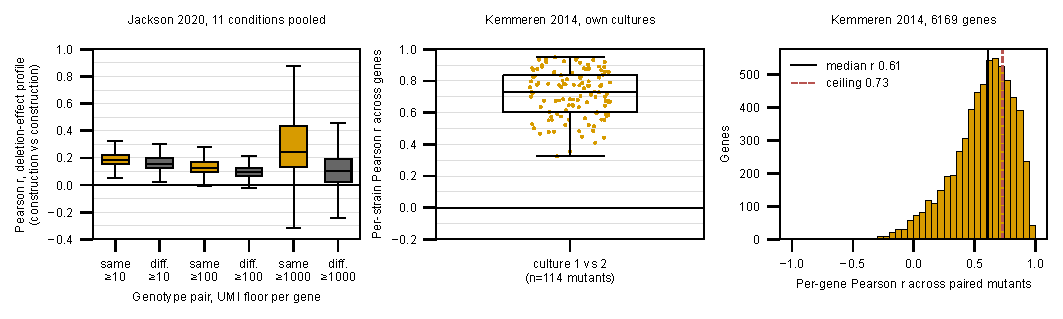
\includegraphics[width=\textwidth]{figures/within_dataset_ceilings_2026-10-19-16-49-03.pdf}\par\vspace{2pt}
\caption[]{\textbf{Two datasets measured against themselves.} \textbf{a}, Jackson 2020:
Pearson over genes of the deletion-effect profiles of two constructions in one condition,
same genotype (orange) against different genotypes (gray), at three floors on a gene's
UMIs summed over the condition; 1{,}778 and 21{,}300 pairs per floor, 11 conditions
pooled, HO pairs left out. \textbf{b}, Kemmeren 2014: Pearson across genes between the two
cultures of each of the 114 mutants profiled twice; culture 1 of one mutant against
culture 2 of another gives a median of 0.284 (not drawn). \textbf{c}, per-gene Pearson
across the 114 mutants for 6{,}169 genes, with the median $r$ and the ceiling, the mean
over genes of $\sqrt{\max(r_g, 0)}$.}
\label{fig:ceilings}
\end{figure}
%% Generated by experiments/043-expression-proteome-morphology/scripts/within_dataset_ceilings.py

\begin{figure}[htbp]\centering
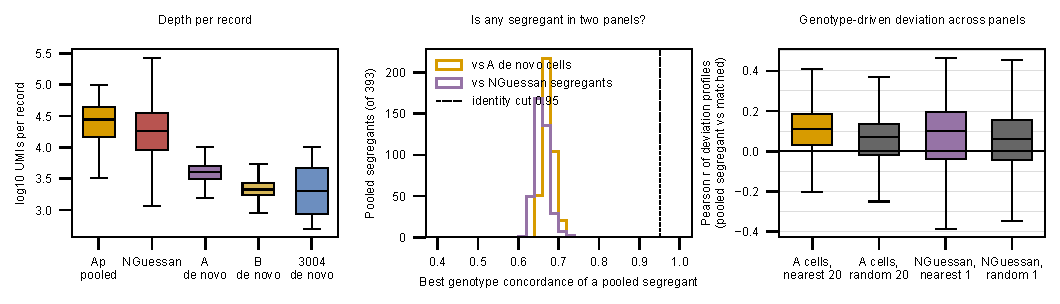
\includegraphics[width=\textwidth]{figures/within_dataset_segregants_2026-10-19-16-49-04.pdf}\par\vspace{2pt}
\caption[]{\textbf{The segregant panels have no shared segregant and a weak shared
genotype signal.} \textbf{a}, UMIs per record by panel (pooled records sum a segregant's
cells, de novo records are single cells). \textbf{b}, for each of the 393 pooled Boocock
segregants, the best genotype concordance with any de novo cross-A cell (orange) or any
N'Guessan segregant (purple), on a 5 kb grid of called parents; the dashed line marks
0.95. \textbf{c}, Pearson over genes between a pooled segregant's deviation from its
panel and that of its 20 nearest de novo cells, 20 random cells, its nearest N'Guessan
segregant, or a random one; genes with at least 10 UMIs on both sides.}
\label{fig:segregants}
\end{figure}
%% Generated by experiments/043-expression-proteome-morphology/scripts/within_dataset_ceilings.py

\subsection{Between datasets\secstatus{todo}}
\label{sec:between}

Records are matched by perturbed gene names and environment (isolates by strain name),
and each pair is scored per shared genotype, across shared genes, and per shared gene,
across shared genotypes (Table~\ref{tab:cross}, Fig.~\ref{fig:pergenotype};
\file{experiments/043-expression-proteome-morphology/scripts/cross_dataset_correlation.py},
slurm jobs 5890 and 5892). Every pair compares log against log, so the base of a
logarithm does not change a correlation.

%% SOURCE: experiments/043-expression-proteome-morphology/scripts/primer_043_tables.py
%% -> tables/t7-cross.tex
\begin{table}[htbp]
\centering
\scriptsize
\setlength{\tabcolsep}{3pt}
\caption[]{\textbf{Agreement between datasets of the same readout type.} Per genotype:
Pearson and Spearman across the shared genes (at least 20). Per gene: Pearson across the
shared genotypes (at least 5). Jackson is turned into a deletion effect against HO in the
same environment; Messner and Zelezniak are log ratios to their record reference; Caudal
and Muenzner are centered per gene over the isolates. The Jackson environment row pairs
one genotype across two environments (605 genotype-environment pairs).}
\label{tab:cross}
%% GENERATED by experiments/043-expression-proteome-morphology/scripts/primer_043_tables.py
%% SOURCE: results/store_census.json, results/cross_dataset_correlation.json,
%% results/within_dataset_ceilings.json and the 019 ceiling files named in
%% tables/provenance.json. Do not edit by hand.

\begin{tabular}{>{\raggedright\arraybackslash}p{46mm}>{\raggedleft\arraybackslash}p{16mm}>{\raggedleft\arraybackslash}p{30mm}>{\raggedleft\arraybackslash}p{18mm}>{\raggedleft\arraybackslash}p{26mm}>{\raggedleft\arraybackslash}p{20mm}}
\toprule
Pair & Shared genotypes, n & Per-genotype Pearson r, median [IQR] & Per-genotype Spearman, median & Per-gene Pearson r, median (genes, n) & Genes with per-gene r $>$ 0.3, fraction \\
\midrule
Kemmeren $\times$ Sameith Sm & 82 & 1.000 [1.000, 1.000] & 1.000 & 1.000 (6{,}169) & 1.000 \\
Kemmeren $\times$ Hu & 255 & 0.107 [0.013, 0.184] & 0.082 & 0.097 (5{,}803) & 0.102 \\
Kemmeren $\times$ Nadal, YPD & 913 & 0.002 [$-$0.017, 0.022] & 0.007 & 0.017 (5{,}891) & 0.007 \\
Kemmeren $\times$ Nadal, NaCl & 920 & $-$0.001 [$-$0.021, 0.022] & 0.005 & 0.015 (5{,}896) & 0.006 \\
Kemmeren $\times$ Jackson, YPD 10 h & 11 & 0.043 [0.026, 0.070] & 0.047 & 0.035 (5{,}340) & 0.247 \\
Kemmeren $\times$ Jackson, YPD 4 h (a) & 11 & 0.066 [0.027, 0.210] & 0.030 & 0.118 (5{,}353) & 0.321 \\
Kemmeren $\times$ Jackson, YPD 4 h (b) & 11 & 0.076 [0.036, 0.149] & 0.045 & 0.052 (5{,}601) & 0.253 \\
Nadal YPD $\times$ Nadal NaCl & 2{,}952 & 0.208 [0.168, 0.231] & 0.043 & 0.183 (6{,}134) & 0.050 \\
Nadal duplicates, one condition & 105 & 0.376 [0.323, 0.452] & 0.178 & 0.062 (5{,}897) & 0.089 \\
Jackson, environment $\times$ environment & 605 & 0.010 [$-$0.005, 0.029] & 0.009 & n/a & n/a \\
Messner $\times$ Zelezniak (protein) & 89 & 0.049 [$-$0.016, 0.185] & 0.050 & 0.085 (715) & 0.067 \\
Kemmeren mRNA $\times$ Messner protein & 1{,}349 & 0.031 [$-$0.025, 0.112] & 0.034 & 0.094 (1{,}832) & 0.033 \\
Caudal mRNA $\times$ Muenzner protein & 759 & 0.208 [0.109, 0.307] & 0.176 & 0.160 (1{,}572) & 0.183 \\
Muenzner turnover $\times$ abundance & 55 & $-$0.006 [$-$0.053, 0.047] & $-$0.003 & $-$0.007 (1{,}120) & 0.066 \\
\bottomrule
\end{tabular}

\end{table}

\notesec{Sameith 2015 single mutants are Kemmeren 2014's arrays}
All 82 Sameith Sm profiles are value-for-value identical to Kemmeren's for the same
deletions (median per-genotype $r$ = 1.000), and the GEO deposits show why. GSE42536
holds 144 Sameith single-mutant arrays: 115 are byte-identical re-deposits of GSE42527 or
GSE42526 arrays, and the other 29 match a Kemmeren array exactly on the normalized Cy5
and Cy3 signal columns. Sameith's Methods defer to the earlier paper: ``Full details of
all gene expression profiling procedures have been described before [46]''. The pair is
therefore no replicate, and the experiment 019 expression ceiling built on it
(test-retest 0.744 per strain, ceiling 0.77) is void; Table~\ref{tab:kemmeren} replaces
it. The 143 Sameith double-mutant arrays are new hybridizations.

\notesec{Nadal-Ribelles 2025}
Nadal-Ribelles agrees with Kemmeren at a median per-genotype $r$ of 0.002 in YPD (913
deletions) and with itself not much better. Experiment 028 measured the same genotype
across batches at a median $r$ of 0.043 against 0.022 for different genotypes, and
split halves at 0.080 against 0.051. The 0.376 of within-condition duplicates in
Table~\ref{tab:cross} is Pearson driven by a few extreme log fold changes (the Spearman
of the same pairs is 0.178); hypothesis, untested, that they come from genes with
near-zero counts on one side.

\notesec{Jackson 2020 across environments}
One TF deletion's effect profile in one environment agrees with the same deletion's
profile in another at a median $r$ of 0.010 (605 pairs). The paper reports that TF
deletions change far fewer genes than conditions do (96 differentially expressed genes in
YPD, 160 in rapamycin), so a near-zero cross-environment agreement is what the paper
leads one to expect; it does not show the data to be noise, and the within-condition
construction pairs above measure the noise directly.

\notesec{mRNA against protein}
Deletions agree weakly: Kemmeren against Messner gives a median per-genotype $r$ of 0.031
over 1{,}349 deletions and a per-gene $r$ of 0.094 over 1{,}832 genes. Isolates agree
more: Caudal against Muenzner gives 0.208 over 759 isolates and 0.160 per gene. Protein
varies far more across isolates than across deletions (Fig.~\ref{fig:mrnaprot}, left, x axes); hypothesis, untested, that this larger range is why the two readouts agree more
there. Turnover against abundance is near zero (55 isolates).

\notesec{Expression to morphology}
A ridge from each gene-level matrix to the 281 CalMorph features of the shared Ohya
genotypes (5-fold out-of-fold, one row-permutation null) is the one cross-label link that
matters for a held-out probe (Table~\ref{tab:morph}, Fig.~\ref{fig:mrnaprot}, right). Kemmeren
carries the most signal per genotype; Messner reaches nearly as far on three times the
genotypes.

%% SOURCE: experiments/043-expression-proteome-morphology/scripts/primer_043_tables.py
%% -> tables/t8-morphology.tex
\begin{table}[htbp]
\centering
\footnotesize
\caption[]{\textbf{Ridge from a gene-level matrix to CalMorph.} Out-of-fold Pearson per
CalMorph feature across held-out genotypes; inputs and targets z-scored and clipped at 8,
penalty chosen on an inner split. The 116 moving features are the experiment 019 list
(\file{calmorph_moving_features.json} on the multimodal-phenotype-retrospective
worktree).}
\label{tab:morph}
%% GENERATED by experiments/043-expression-proteome-morphology/scripts/primer_043_tables.py
%% SOURCE: results/store_census.json, results/cross_dataset_correlation.json,
%% results/within_dataset_ceilings.json and the 019 ceiling files named in
%% tables/provenance.json. Do not edit by hand.

\begin{tabular}{>{\raggedright\arraybackslash}p{30mm}>{\raggedleft\arraybackslash}p{26mm}>{\raggedleft\arraybackslash}p{26mm}>{\raggedleft\arraybackslash}p{26mm}>{\raggedleft\arraybackslash}p{26mm}}
\toprule
Input matrix & Genotypes shared with Ohya, n & Mean r over 281 features & Row-permutation null, mean r & Median r over 116 moving features \\
\midrule
Kemmeren 2014 & 1{,}437 & 0.238 & $-$0.005 & 0.348 \\
Messner 2023 & 4{,}279 & 0.179 & 0.008 & 0.278 \\
Hu 2007 & 259 & 0.114 & $-$0.052 & 0.235 \\
Sameith 2015 Sm & 81 & $-$0.014 & $-$0.077 & $-$0.085 \\
\bottomrule
\end{tabular}

\end{table}

%% SOURCE: experiments/043-expression-proteome-morphology/scripts/cross_dataset_correlation.py
%% -> figures/cross_dataset_per_genotype_pearson_2026-10-19-14-37-41.pdf, figures/cross_dataset_mrna_protein_per_gene_2026-10-19-14-37-41.pdf, figures/cross_dataset_morphology_ridge_2026-10-19-14-37-41.pdf
\begin{figure}[htbp]\centering
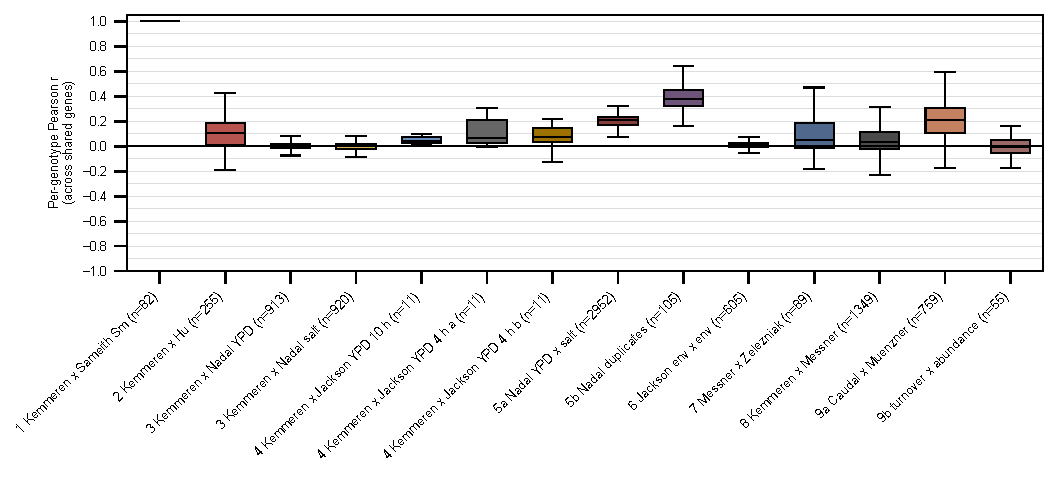
\includegraphics[width=\textwidth]{figures/cross_dataset_per_genotype_pearson_2026-10-19-14-37-41.pdf}\par\vspace{2pt}
\caption[]{\textbf{Agreement between datasets is low except for the Sameith copy.} Per
shared genotype, Pearson across the shared genes for every pair of Table~\ref{tab:cross};
boxes are quartiles, whiskers 1.5 IQR, outliers not drawn.}
\label{fig:pergenotype}
\end{figure}
%% Generated by experiments/043-expression-proteome-morphology/scripts/cross_dataset_correlation.py

\begin{figure}[htbp]\centering
\begin{minipage}[b]{0.49\textwidth}\centering
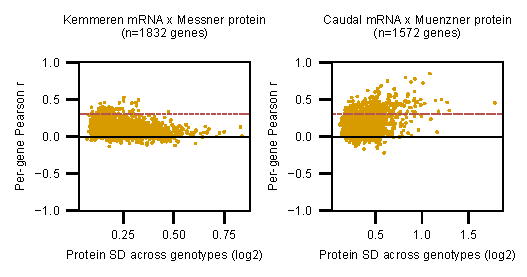
\includegraphics[width=\linewidth]{figures/cross_dataset_mrna_protein_per_gene_2026-10-19-14-37-41.pdf}
\end{minipage}\hfill
\begin{minipage}[b]{0.49\textwidth}\centering
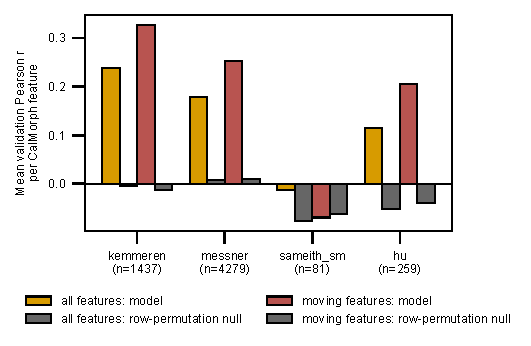
\includegraphics[width=\linewidth]{figures/cross_dataset_morphology_ridge_2026-10-19-14-37-41.pdf}
\end{minipage}\par\vspace{2pt}
\caption[]{\textbf{mRNA against protein, and expression to morphology.} Left two panels:
per-gene Pearson between mRNA and protein across the shared genotypes, against the
protein's SD across those genotypes, for 1{,}832 genes over the deletions of Kemmeren and
Messner and 1{,}572 genes over the isolates of Caudal and Muenzner; the dashed line marks
$r$ = 0.3. Right: mean out-of-fold Pearson per CalMorph feature of a ridge from each input
matrix (Table~\ref{tab:morph}), with its row-permutation null.}
\label{fig:mrnaprot}
\end{figure}
%% Generated by experiments/043-expression-proteome-morphology/scripts/cross_dataset_correlation.py

%% notes-tex/multimodal/043-datasets-primer/sections/4-colocation.tex

\section{Which genotypes carry which labels\secstatus{todo}}
\label{sec:colocation}

A multitask model learns a shared representation only where one genotype carries more
than one label. The census keys a genotype by its perturbed gene names, an isolate by its
strain and a segregant by cross and identifier, and counts the genotypes each label and
each pair of labels reach (Tables~\ref{tab:bylabel} and~\ref{tab:coloc}).

%% SOURCE: experiments/043-expression-proteome-morphology/scripts/primer_043_tables.py
%% -> tables/t10-by-label.tex and tables/t9-colocation.tex
\begin{table}[htbp]
\centering
\footnotesize
\begin{minipage}[t]{0.36\textwidth}\centering
\caption[]{\textbf{Genotypes per label.} Distinct genotype keys over every dataset
carrying the label; Vaishnav is not keyed by gene and is left out.}
\label{tab:bylabel}
%% GENERATED by experiments/043-expression-proteome-morphology/scripts/primer_043_tables.py
%% SOURCE: results/store_census.json, results/cross_dataset_correlation.json,
%% results/within_dataset_ceilings.json and the 019 ceiling files named in
%% tables/provenance.json. Do not edit by hand.

\begin{tabular}{>{\raggedright\arraybackslash}p{40mm}r}
\toprule
Label & Genotypes, n \\
\midrule
umi\_count & 82{,}479 \\
protein\_abundance & 5{,}279 \\
calmorph & 4{,}678 \\
expression\_log2\_ratio & 3{,}685 \\
expression\_tpm & 943 \\
expression\_score & 262 \\
degradation\_rate & 55 \\
\bottomrule
\end{tabular}

\end{minipage}\hfill
\begin{minipage}[t]{0.6\textwidth}\centering
\caption[]{\textbf{Co-location.} Genotypes carrying both labels, in any datasets. A
label name can span datasets: \texttt{expression\_log2\_ratio} is Kemmeren, Sameith and
Nadal-Ribelles; \texttt{umi\_count} is Jackson, Boocock and N'Guessan;
\texttt{protein\_abundance} is Messner, Zelezniak and Muenzner.}
\label{tab:coloc}
%% GENERATED by experiments/043-expression-proteome-morphology/scripts/primer_043_tables.py
%% SOURCE: results/store_census.json, results/cross_dataset_correlation.json,
%% results/within_dataset_ceilings.json and the 019 ceiling files named in
%% tables/provenance.json. Do not edit by hand.

\begin{tabular}{>{\raggedright\arraybackslash}p{80mm}r}
\toprule
Labels carried by the same genotype & Genotypes, n \\
\midrule
expression\_log2\_ratio $\times$ calmorph & 3{,}473 \\
protein\_abundance $\times$ calmorph & 4{,}287 \\
expression\_log2\_ratio $\times$ protein\_abundance & 3{,}317 \\
expression\_tpm $\times$ protein\_abundance & 759 \\
umi\_count $\times$ calmorph & 12 \\
expression\_score $\times$ calmorph & 259 \\
isolates: Caudal $\times$ Muenzner protein & 759 \\
isolates: all three isolate datasets & 55 \\
\bottomrule
\end{tabular}

\end{minipage}
\end{table}

\notesec{Deletions}
Morphology is the label most often shared. Of the 4{,}678 CalMorph genotypes, 4{,}287
also carry a protein profile and 3{,}473 an expression log ratio; the
expression-by-protein overlap is 3{,}317 genotypes. That count includes Nadal-Ribelles,
whose within-dataset agreement is near its null (Sec.~\ref{sec:within}); Kemmeren alone
shares 1{,}349 genotypes with Messner. Kemmeren reaches Ohya on 1{,}437
genotypes and Messner on 4{,}279, the populations of the morphology ridge
(Table~\ref{tab:morph}).

\notesec{Isolates}
The isolate datasets are nested: all 55 turnover isolates are in the protein set and in
Caudal's transcriptomes, and 759 of the 795 protein isolates have a Caudal
transcriptome. No isolate carries a CalMorph profile.

\notesec{Segregants and the rest}
No segregant shares a key with any other dataset, and Boocock and N'Guessan share no
segregant with each other (0 shared identifiers; Sec.~\ref{sec:within} tests genotype
identity rather than names). The 12 \texttt{umi\_count} genotypes that carry morphology
are Jackson's 11 transcription-factor deletions and the HO control.

%% notes-tex/multimodal/043-datasets-primer/sections/5-proposal.tex
%% SOURCE: the owner's direction of 2026-10-19 (notes/experiments.043-expression-proteome-morphology.md,
%% "Design pass") and the 2026-10-20 review pass (same note, "Review pass"); numbers from
%% results/data_shapes_043.json, results/store_census.json, results/cross_dataset_correlation.json,
%% results/within_dataset_ceilings.json and results/distinct_alleles.json, through the tables
%% written by experiments/043-expression-proteome-morphology/scripts/primer_043_tables.py. The
%% case-study numbers cite their experiment's records: 031 (memory 031-inductive-fold-program,
%% jobs 5022 to 5081; operator audit jobs 4917 and 4918; closure plan header), 035 (rounds 2,
%% 9 to 11, slurm 3034, 3009) and 038 (slurm 3374, 3700, 3701), 010 and 030
%% (notes-tex/trigenic/010-additive-baselines; job 1605; job 3902; W&B xy3xnpau).

\section{The plan: every gene-level readout trained together\secstatus{todo}}
\label{sec:proposal}

Every gene-level readout of the store trains in one model, and the question it answers
is an engineering one: does the model predict the transcriptome of a deletion it has not
seen, and of a double deletion from its two measured singles? Table~\ref{tab:plan} gives
the sets. An earlier version of this section proposed two separate training batches,
deletions and then isolates with segregants; the owner superseded it on 2026-10-19, and the
review pass of 2026-10-20 replaced the separate split draws by one fold file and put a
linear ladder and a decision rule ahead of any training run.

%% SOURCE: experiments/043-expression-proteome-morphology/scripts/primer_043_tables.py
%% -> tables/t11-plan.tex (record counts from results/data_shapes_043.json and store_census.json)
\begin{table}[htbp]
\centering
\footnotesize
\caption[]{\textbf{The sets of the plan.} Records count the raw store (full pass of
\file{data_shapes_043.py}, slurm job 5902). The fold file is not yet written, so a split's
count is its expected fold-0 share under the stratified draw: a tenth of each deletion
dataset's genes, a fifth of the isolates by strain name, of each segregant panel and of the
promoter variants. Splits A, C, D and E are carved out of training records; split B is a
dataset of its own and never trains.}
\label{tab:plan}
%% GENERATED by experiments/043-expression-proteome-morphology/scripts/primer_043_tables.py
%% SOURCE: results/store_census.json, results/cross_dataset_correlation.json,
%% results/within_dataset_ceilings.json and the 019 ceiling files named in
%% tables/provenance.json. Do not edit by hand.

\begin{tabular}{>{\raggedright\arraybackslash}p{30mm}>{\raggedright\arraybackslash}p{52mm}>{\raggedleft\arraybackslash}p{16mm}>{\raggedright\arraybackslash}p{72mm}}
\toprule
Set & Datasets & Records or held-out units, n (expected) & Role \\
\midrule
Training, every gene-level readout & Kemmeren 2014, Hu 2007, Jackson 2020, Nadal-Ribelles 2025, Messner 2023, Zelezniak 2018, Caudal 2024, Muenzner 2024 protein, Muenzner 2024 turnover, Boocock 2025, N'Guessan 2025, Vaishnav 2022 & 168{,}785 & trained together; fold 0 of each key space is carved out of these records, fold 1 validates \\
Split A, deletion genes & every deletion dataset & 140 & gene fold 0: about a tenth of Kemmeren's 1{,}400 genes outside the 82 pinned Sameith singles; also Messner 2023 about 448, Nadal-Ribelles 2025 about 306, Hu 2007 about 26, Zelezniak 2018 about 10, Ohya 2005 about 468 \\
Split B, Sameith doubles & Sameith 2015 Dm & 72 & every double; scored against the per-gene mean, the stronger single, the additive null and the fitted combination of its singles \\
Split C, isolates & Caudal 2024, Muenzner 2024 protein and turnover & 196 & isolate fold 0 of 979 strains: about 159 Muenzner and 11 turnover isolates, out of every readout \\
Split D, segregants & Boocock 2025, N'Guessan 2025 & 16{,}493 & fold 0 within each cross: about 15{,}903 Boocock and 590 N'Guessan records \\
Split E, promoters & Vaishnav 2022 & 14{,}232 & fold 0 of 71{,}158 promoter variants; linear evaluations first \\
Probe & Ohya 2005 & 4{,}678 & ridge from the frozen latent to the CalMorph features, raw and growth-residualized; never trained \\
Dropped & Sameith 2015 Sm & 82 & the same arrays as Kemmeren (82 of 82) \\
\bottomrule
\end{tabular}

\end{table}

\notesec{Training}
Twelve datasets train together: every dataset of the store except Sameith 2015 Sm,
whose 82 profiles are Kemmeren's own arrays (82 of 82 identical), Sameith 2015 Dm, which
is split B, and Ohya 2005, which is the probe. Vaishnav 2022 stays in the plan as the
promoter signal: one sort-seq level per promoter insert, read at the record level through
the reporter token of Sec.~\ref{sec:input-token}, whose promoter block is the frozen FUDT
upstream encoder on the construct window; its linear evaluations run first and its joint
entry waits on the Addgene 127546 sequence. Expression and protein readouts come off the
perturbed graph: a gene's value is read from that gene's own perturbed node state, and the
CLS state and the perturbed-gene summary $z_S$ are the record-level sites
(Sec.~\ref{sec:output-sites}). The low-agreement datasets train too, and their measured
agreement is what the arm without them reads: Nadal-Ribelles agrees with itself across
batches at a median $r$ of 0.043 against 0.022 for different genotypes and with Kemmeren
at 0.002; two Jackson 2020 constructions of one genotype agree at 0.129 against 0.095; Hu
2007 released no replicate and agrees with Kemmeren at 0.107 per genotype, on an X score
that is not a log ratio; Zelezniak 2018 agrees with Messner at 0.049 per genotype over 715
proteins though its own ceiling is 0.916; Muenzner 2024 turnover agrees with abundance at
$-$0.006 per isolate.

\notesec{Split A, deletion genes}
One fold file holds every deletion gene's fold; fold 0 is held out of every deletion
dataset at once, so a held-out gene is never seen as a perturbation on any readout, and
the same genes test Kemmeren, Messner, Hu, Nadal-Ribelles and Zelezniak alone and jointly.
Kemmeren holds out about 140 of its 1{,}400 eligible genes (the 82 Sameith singles are
pinned to training). The score is the median per-gene Pearson across those strains; the
per-strain Pearson is reported centered, because two different Kemmeren mutants already
agree at a raw 0.284 (Sec.~\ref{sec:within}). The bound is Kemmeren's own-culture ceiling,
0.729 over 114 mutants with two cultures; the bars are the frozen-token ridge and kNN of
Sec.~\ref{sec:output-linear} on the same genes.

\notesec{Split B, the Sameith doubles}
All 72 Sameith 2015 double deletions are held out and scored, centered, against their
measured profiles and against four rungs that need no model: the per-gene mean, the
stronger single, the additive null of the two Kemmeren singles (the paper's own expected
value) and a fitted combination of the two singles. Sameith's Methods defer to Kemmeren's,
so the doubles were profiled by the same procedure; no double has a replicate, and the
Kemmeren ceiling of 0.729 is the bound for the same arrays.

\notesec{Split C, the isolates}
Fold 0 of the isolate folds, about 196 of the 979 Caudal and Muenzner strains with about
159 Muenzner and 11 turnover isolates among them, is held out of every readout of those
isolates. The bar is kinship ridge (GBLUP) on the same isolates; the reference is how far
another readout of the same isolate agrees, Caudal mRNA against Muenzner protein at a
median per-isolate $r$ of 0.208, against 0.031 for Kemmeren mRNA against Messner protein on
deletions. Splits D (segregants, within cross) and E (promoters) come from the same file.

\notesec{The morphology probe}
Ohya 2005 CalMorph enters no training. Its 4{,}678 genotypes are run through the frozen
model and a ridge reads the 116 moving features from $h$, $z_S$, $\bar H$ and their
concatenation, raw and with the Costanzo single-mutant fitness regressed out, since growth
matrices alone predict morphology nearly as well as the proteome (019 screen). A ridge on
the measured inputs already reaches a median $r$ of 0.348 from Kemmeren expression
(1{,}437 shared genotypes), 0.278 from Messner protein (4{,}279) and 0.235 from Hu (259)
over the 116 moving features, against row-permutation nulls near zero, and Ohya's own
ceiling is 0.611 over 122 wild-type replicates on all 281 (Table~\ref{tab:morph}).
Sec.~\ref{sec:output-protocol} gives the bars and the two reads.

\notesec{The genotypes the model has not yet read}
Isolates and segregants need a gene-level genotype the \texttt{Perturbation} processor
does not build: marking every isolate perturbation sets 5{,}575 of 6{,}607 nodes, and a
segregant sets none. Sec.~\ref{sec:input} gives the replacement: each isolate as its own
reference context built from its allele embeddings, with an interim arm that marks loss of
function and absence on S288C, and the definite rule for segregants (a gene inherits the
non-reference parent only inside a block called at posterior 0.9 or above), with the
parent's real allele token. The posterior cut removes little on the pooled panels (a
median of 0\% of markers for Boocock pooled, 1.7\% for N'Guessan) and a quarter to a third
on Boocock's de novo cells, whose single cells carry medians of 2{,}000 to 4{,}000 UMIs;
whether those cells train is decision P1. The measured genotype signal across segregant
panels is small: nearest-genotype deviation $r$ 0.113 against 0.070 for random pairs
(Sec.~\ref{sec:within}).

\subsection{What the three case studies teach\secstatus{todo}}
\label{sec:lessons}

Three earlier campaigns trained the same cell graph transformer on other labels, and each
found a bar, a scoring trap and a protocol that the first 043 design did not carry.

\notesec{Betaxanthin, experiment 031}
The GO recipe with a rank term reached a fold-average held-out Spearman of 0.229 to 0.230
over six seeds (fold sd 0.003 to 0.006), 0.264 on the pinned fold; the annotation-free cell
(composite sequence token plus metabolic block) 0.108 on the fold average and 0.125 on the
pin. The bars were ridge on the deleted gene's raw ProtT5 token, 0.082 on the pin, and
forests on ProtT5 (0.150) and on GO plus pFBA (0.204) on the fold average. What made it
honest: five inductive folds over deletion genes with the external pin as fold 0, every arm
paired by seed against a named control, the rule of a gain of at least 0.02 with 5 of 6
seeds up (9 of 12 at twelve), and a fixed budget, since epoch selection on validation was
null ($-0.009$). The operator audit (jobs 4917, 4918) found the single-deletion score to be
a learned affine read of the deleted gene's own token, reproduced by a ridge from that row:
the inductive gap is in the representation, not the head. Split A is a single-deletion task
and the same audit applies, so the first number to produce is the ridge from the deleted
gene's frozen composite token to its profile; the first 043 design ran no such bar and
proposed three initializations by two split seeds with no fold structure, where 031 found
the pin's sampling sd (0.041) equal to the seed sd.

\notesec{Environment, experiments 035 and 038}
Nested ridge on raw FCFP4 counts reached a median centered Spearman per held-out compound
of 0.303 over 123 compound-evaluations (035, slurm 3034) and 0.359 over 96 on the second
build (038, slurm 3374); the transformer trained to saturation tied ridge on the first
build (every entry point's compound-level interval through zero) and sat below it on the
second (0.312 and 0.297; slurm 3700, 3701). The protocol that fixed the verdict: fit on the
whole non-test pool as ridge does, a fixed 50 epochs keeping the last, three seeds, paired
against ridge on the same held-out units, and the interval resampled over the 41 compounds
rather than the 123 evaluations. Its centering lesson: each side is centered by its own
training mean, since centering the prediction by the measured mean rewarded an untrained
model at 0.356 after 60 steps (slurm 3009). The per-strain Pearson across genes has the
same trap here: Kemmeren's different-mutant pairs agree at 0.284 (job 5893), the shared
deletion response, which a model that emits the training-mean profile earns. Every
per-strain Pearson is therefore reported centered, and the per-gene mean is the first rung.

\notesec{Trigenic, experiments 010 and 030}
The trigenic Pearson reached $0.454 \pm 0.006$ on the random split and fell to about 0.13
for every model on held-out query pairs, with the fitness-head model recovering 0.41 on one
seed. On the random split the ladder read 0.390 for the query pair alone, 0.400 for the
additive per-gene ridge, 0.425 to 0.427 for an embedding MLP and 0.438 to 0.455 for the
transformer; on the 030 pool a zero-parameter lower-order null read 0.577 and 0.566 and
boosted trees over the lower-order terms 0.743 and 0.700, above the joint transformer's
0.562 and 0.391 (job 3902). The per-entry dataset token (a 15-way one-hot projected to 8
dimensions at the readout) converged at a validation interaction Pearson of 0.5655 on one
seed. Ordering generalized and magnitudes did not (held-out calibration slope 0.24, job
1605), and the slope is a property of the population scored (0.88 on the whole test split
against 1.59 inside the predicted top 100). Split B carries the additive null but needs the
whole ladder of rungs that see only a double's components, and because the binned head's
point prediction is an expectation that shrinks toward the mean, Spearman sits beside
Pearson and the calibration slope is named by population.

\notesec{The unified protocol}
Four steps, in order. (1) The linear ladder on CPU from the frozen embeddings, on the same
held-out units the transformer will use (Sec.~\ref{sec:output-linear}); nothing trains on a
card until it is on file. (2) The rule, committed as \file{conf/decision\_rule.yaml} before
the first GPU run: primary statistic per split, the control arm, a gain of at least 0.02,
at least 5 of 6 paired seeds up, and a 95\% interval resampled over held-out strains (genes
for per-gene statistics) that excludes zero. (3) Training with the budget and window
declared at launch; the validation fold monitors the escape and never selects the epoch;
the test fold is read once. (4) Paired comparison by initialization seed, each arm against
its named control, at the unit of generalization: held-out deletion gene, isolate, double,
segregant or promoter, with both intervals computed and the unit-level one quoted.

\notesec{Decisions}
Table~\ref{tab:decisions} collects every choice the design leaves to the owner, with
two options, the measured fact that bears on it and the reconciled proposal with its
named alternatives. The I rows come from the input side (Sec.~\ref{sec:input-decisions}),
the O rows from the output side (Sec.~\ref{sec:output-decisions}), the P rows from putting
the plan together, the S rows from the protocol the review pass added, D1 from the data per
model part (Sec.~\ref{sec:data-per-part}) and E1 from the isolate embedding plan
(Sec.~\ref{sec:input-embeddings}).

%% SOURCE: experiments/043-expression-proteome-morphology/scripts/primer_043_tables.py
%% -> tables/t13-decisions-rows.tex (DECISIONS, numbers filled by facts() from the result files)
\begin{landscape}
\scriptsize
\setlength{\tabcolsep}{3pt}
\begin{longtable}{>{\raggedright\arraybackslash}p{6mm}>{\raggedright\arraybackslash}p{22mm}>{\raggedright\arraybackslash}p{44mm}>{\raggedright\arraybackslash}p{30mm}>{\raggedright\arraybackslash}p{56mm}>{\raggedright\arraybackslash}p{62mm}>{\raggedright\arraybackslash}p{9mm}}
\caption[]{\textbf{Owner decisions, one checklist.} Each row is one choice the design
cannot make alone. Option 1 is the reconciled main option; the proposed column states the
decision and names its alternatives; ``open'' marks a choice with no proposal. The
measured fact is the one its section cites. The last column is the section that carries
the full argument.}\label{tab:decisions}\\
\toprule
Id & Decision & Option 1 & Option 2 & Measured fact & Proposed, with alternatives & Sec. \\
\midrule
\endfirsthead
\toprule
Id & Decision & Option 1 & Option 2 & Measured fact & Proposed, with alternatives & Sec. \\
\midrule
\endhead
%% GENERATED by experiments/043-expression-proteome-morphology/scripts/primer_043_tables.py
%% SOURCE: the owner-decision lists of sections/input-design.tex and
%% sections/output-design.tex, condensed in DECISIONS. Do not edit by hand.
I1 & Base gene token & learned identity table (the 019 model) & frozen sequence encoder (ProtT5, nucleotide-transformer windows, FUDT) & every encoder is already a per-gene row on main; the 019 campaign used none; no comparison on expression measured & open & \ref{sec:input-decisions} \\
I2 & Absence and deletion & one change type & two change types & 135 natural absences per Caudal isolate; the similarity is measurable after training as the cosine of the two embeddings & two & \ref{sec:input-decisions} \\
I3 & Isolate marks in the mask & every type, $M\approx$ 5,565 & loss of function and absence, $M\approx$ 518 & operator cost scales with the largest $M$ in a batch; within-isolate mRNA-protein agreement 0.208 does not separate the two & open & \ref{sec:input-decisions} \\
I4 & Segregant gene membership & whole gene inside a block & gene midpoint inside a block & blocks end at marker positions and the crossover lies in the gap; straddling genes per segregant not counted & whole gene (the prototype) & \ref{sec:input-decisions} \\
I5 & Chromosomal position & on for every genotype class & on only when segregants enter & no run bears on it; nearest-genotype deviation $r$ 0.113 against 0.070 is the only segregant signal & open & \ref{sec:input-position} \\
I6 & Strain tokens & extra keys of the operator & added to the CLS row & at $M={}$1 an extra key makes $M={}$2 and changes the softmax, which confounds a comparison with 019 & extra keys (the prototype's layout) & \ref{sec:input-decisions} \\
I7 & Operator normalization at large M & softmax, magnitude fixed & sigmoid gate, magnitude grows with M & operator A run at $M={}$1 to 3 only; sigmoid gate 0.200 against 0.210, one seed; nothing at $M$ of 10 or more & open & \ref{sec:input-decisions} \\
I8 & Accessory ORFs and the Vaishnav reporter & encode each as an extra token & report and skip & 84 accessory presences per Caudal isolate; one reporter (YFP) for 71,158 Vaishnav records & skip accessory ORFs; encode the reporter, since Vaishnav trains & \ref{sec:input-decisions} \\
O1 & Heads & joined by readout type, 6 heads with 15 per-dataset affines & one head per dataset, 15 heads & same-type agreement 0.002 to 0.107 (expression), 0.049 (protein); an affine cannot raise a correlation; no joint training scored & joined; split as the control arm & \ref{sec:output-decisions} \\
O2 & Experiment-type token & flat id & ontology path & the served ontology is flat, 34 leaves under phenotype & flat now, path when the ontology carries one & \ref{sec:output-decisions} \\
O3 & Where the tokens enter & at the head only & on the CLS row, or as an attended token & experiment 035: $-0.007$, $-0.025$, $+0.008$ against ridge for the three forms, every CI through zero & head only; attended token as an arm & \ref{sec:output-decisions} \\
O4 & Loss & MSE & 19-quantile pinball & 019 morphology: MSE on $z_S$ escaped 12 of 12 runs, pinball 8 of 10 & MSE; pinball as an arm & \ref{sec:output-decisions} \\
O5 & Dataset weighting & equal per dataset & by ceiling, or by record count & Boocock and Vaishnav hold 87\% of the records; Kemmeren holds 1,482 & equal, agreement-weighted for the low-agreement sets; record count as an arm & \ref{sec:output-decisions} \\
O6 & Nadal-Ribelles sentinels & $|\log_2\mathrm{FC}|$ > 20 set to missing & keep the stored value & 20.2\% of cells are sentinels & missing & \ref{sec:output-decisions} \\
O7 & Jackson target & deletion effect against the HO control of the same environment & absolute $\log_2(\mathrm{CPM}+1)$ with the environment token & construction pairs agree at 0.129 against 0.095 on the effect; one genotype across environments at 0.010 & the effect & \ref{sec:output-decisions} \\
O8 & Split A leakage rule & held-out gene out of every deletion dataset & out of the expression datasets only & the arm without the natural-genome datasets measures the isolate and segregant side either way & every deletion dataset & \ref{sec:output-decisions} \\
O9 & Split C size & a fifth of the isolates, 159 & another fraction & no Muenzner ceiling; Caudal against Muenzner 0.208 per isolate is the reference & a fifth & \ref{sec:output-decisions} \\
O10 & Budget and window & 019's 500 epochs read over 400 to 499 & a longer budget & 019's 1,000-epoch runs scored lower over 900 to 999 than over 400 to 499 in 7 of 8 & declare with the launch & \ref{sec:output-decisions} \\
P1 & Boocock de novo cells & train all 79,123 single cells under the posterior rule & train the 393 pooled segregants only & de novo cells: median 2,000 to 4,000 UMIs, 24 to 35\% of markers below posterior 0.9 & open; the every-readout direction includes them & \ref{sec:proposal} \\
P2 & Split A against split B & draw split A from Kemmeren genes outside the 82 Sameith singles & draw split A from all 1,482 & split B's additive null needs both singles of each double in training; the overlap of a random draw is not counted & draw outside the Sameith singles & \ref{sec:proposal} \\
\bottomrule

\end{longtable}
\end{landscape}

\notesec{Questions for the owner}
\begin{enumerate}
\item \textbf{Isolates as reference contexts or the interim arm.} The main design encodes
each isolate as its own reference context (979 cached contexts, the operator carrying only
engineered edits) and needs the per-context encoder; the interim arm marks loss of function
and absence on S288C with allele tokens and needs nothing new. Which runs first?
\item \textbf{Addgene 127546.} May its plasmid sequence be fetched into
\file{torchcell-constructs/} with a provenance record, so the Vaishnav construct gets the
1{,}003 bp window the gene promoter encoder expects?
\item \textbf{ProtT5 or ESM2 for the first isolate pass.} 775{,}856 distinct proteins:
about 2.7 hours of ProtT5 on two cards under the stated throughput assumptions, ESM2 about
a third of that.
\item \textbf{Segregant parents.} The five non-BY parents carry Peter ids that are all
members of the gene-keyed allele tarball; confirm that their real allele tokens replace the
parent id on marked genes.
\item \textbf{Headline joint arm.} With or without Hu, Jackson and Nadal-Ribelles (Kemmeren
agreement 0.107, 0.043 to 0.076, 0.002)? They can only lower the Kemmeren score if their
signal does not transfer; the rule names its control before the first read.
\item \textbf{Clade-disjoint isolate split.} A second isolate fold file, disjoint by Peter
2018 clade, beside the random one, once the clade is on the isolate descriptor?
\item \textbf{The quoted per-strain statistic.} Confirm that the centered per-strain
Pearson, with the raw value and the 0.284 floor beside it, is the form quoted.
\end{enumerate}

%% notes-tex/multimodal/043-datasets-primer/sections/6-tensors.tex
%% SOURCE: results/data_shapes_043.json (experiments/043-expression-proteome-morphology/scripts/
%% data_shapes_043.py, slurm job 5902, full pass); the dataset module is
%% experiments/043-expression-proteome-morphology/scripts/dataset_043.py, whose debugger run
%% (six records) is recorded in notes/experiments.043-expression-proteome-morphology.scripts.dataset_043.md.

\section{Data as tensors\secstatus{todo}}
\label{sec:tensors}

Figure~\ref{fig:data-flow} follows a record from the store to a batch, and
Table~\ref{tab:shapes} gives each dataset's shape from a full pass over the 173{,}617
records. A record is a pair of experiment and experiment reference; its genotype becomes
a set of marked genes on the 6{,}607-gene index $G$ of \file{gene_set.json}, its phenotype
a vector $y$ over $G$ with \texttt{NaN} where a gene is not measured, and its environment,
dataset and experiment type become integer tokens.

%% SOURCE: notes/experiments.043-expression-proteome-morphology.mermaid.data-flow.md, rendered by
%% notes/assets/publish/scripts/mermaid_pdf.sh, copied to figures/ by `make diagrams`
\begin{figure}[htbp]\centering
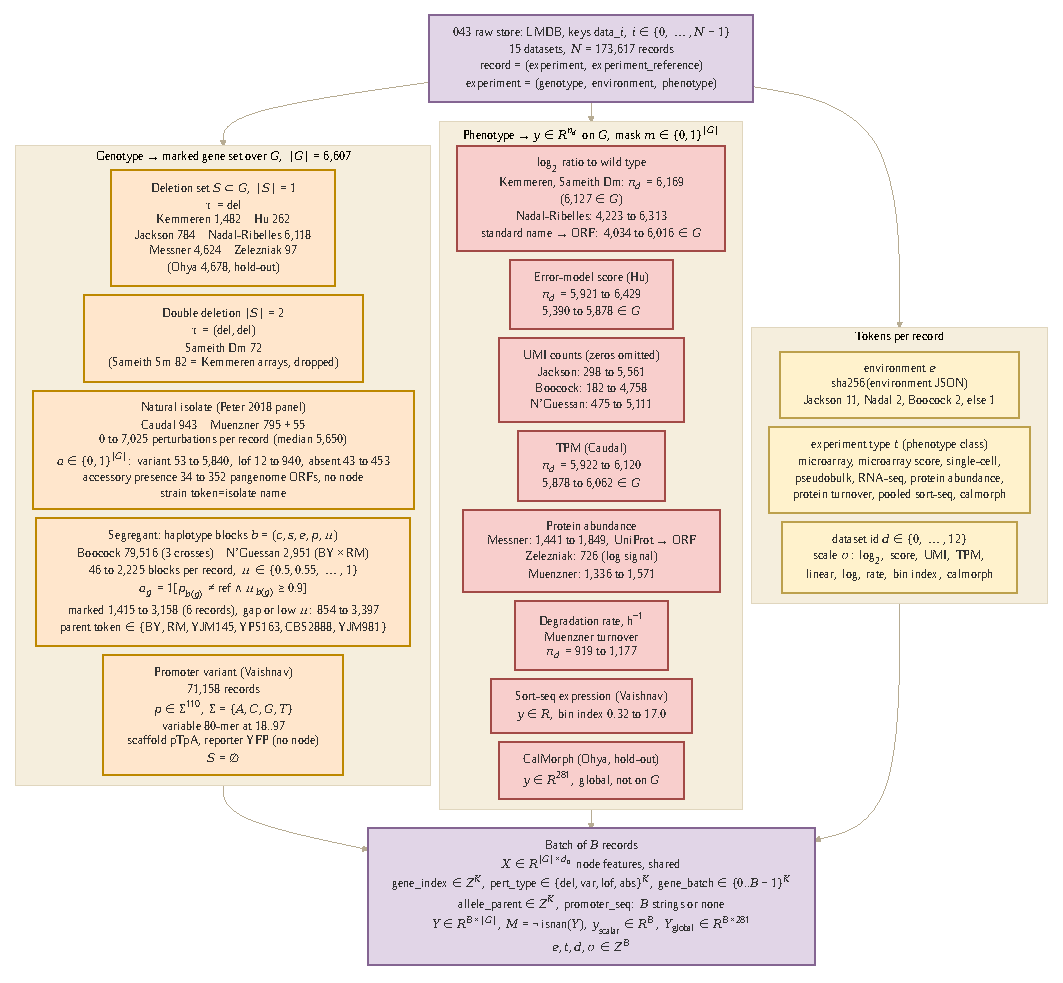
\includegraphics[width=\textwidth]{figures/mermaid-data-flow.pdf}\par\vspace{2pt}
\caption[]{\textbf{A record of the store becomes a marked gene set, a masked label vector
and four tokens.} Left, the five genotype classes and the counts each marks; middle, the
nine released label scales with the number of label keys per record and how many of them
fall on $G$; right, the environment, experiment-type and dataset tokens; bottom, the batch
the collate function returns. Rendered 212 mm wide and placed at 180 mm, a scale of 0.85.}
\label{fig:data-flow}
\end{figure}
%% Generated by notes/assets/publish/scripts/mermaid_pdf.sh from
%% notes/experiments.043-expression-proteome-morphology.mermaid.data-flow.md

\notesec{What the dataset module returns}
Per sample, \file{dataset_043.py} returns the marked genes as indices on $G$
(\file{gene_index}), a change type per marked gene (\file{pert_type}), the allele parent
per marked gene for the segregants (\file{allele_parent}), the promoter sequence and
scaffold for Vaishnav, the environment, dataset and experiment-type ids, the label scale
(\file{y_scale}), the label $y\in\mathbb{R}^{6{,}607}$, one scalar for Vaishnav and the
281 CalMorph features for Ohya. The collate function concatenates the marked genes with a
batch vector and stacks $y$ into a $B\times 6{,}607$ tensor with its measured mask. A
mixed batch of one record per dataset, 15 rows, carries 21{,}728 marked genes, 21{,}713
of them from the five isolate and segregant rows (the six-record debugger run).

\notesec{Three shapes that bear on the design}
The isolate and segregant rows are dense: a Caudal isolate marks 4{,}952 to 5{,}995 of
6{,}607 genes and a segregant 1{,}415 to 3{,}158 under the definite rule, against one
for a deletion, so the perturbation operator sees three orders of magnitude of marked-set
size across datasets (counts on the debugger records). The definite rule leaves gaps: on
the six debugger records 697 to 2{,}693 genes fall between blocks and 157 to 704 under a
block below posterior 0.9. Two label-key maps run at read time: Nadal-Ribelles keys are
standard names (1{,}441 of 6{,}796 on $G$ by raw name, 6{,}325 after the map) and Messner
keys are UniProt accessions (0 of 1{,}850 by raw name, 1{,}850 after). A key with no
position on $G$ is counted per sample and dropped from $y$, never guessed.

%% SOURCE: experiments/043-expression-proteome-morphology/scripts/primer_043_tables.py
%% -> tables/t12-shapes-rows.tex (results/data_shapes_043.json)
\begin{landscape}
\scriptsize
\setlength{\tabcolsep}{3pt}
\begin{longtable}{>{\raggedright\arraybackslash}p{24mm}>{\raggedright\arraybackslash}p{24mm}>{\raggedleft\arraybackslash}p{12mm}>{\raggedright\arraybackslash}p{24mm}>{\raggedleft\arraybackslash}p{20mm}>{\raggedright\arraybackslash}p{31mm}>{\raggedleft\arraybackslash}p{19mm}>{\raggedleft\arraybackslash}p{23mm}>{\raggedleft\arraybackslash}p{23mm}>{\raggedleft\arraybackslash}p{18mm}}
\caption[]{\textbf{Every dataset of the store as tensors.} One row per dataset, from a
full pass over the raw store (\file{data_shapes_043.py}, slurm job 5902). Perturbations
per record count the released perturbation list (a segregant has none; its genotype is a
list of haplotype blocks). Label values are the finite minimum and maximum over a sample
of each dataset's values, on the released scale. Label keys on $G$ count the keys that
land on the 6{,}607-gene index after the read-time maps. Where a cell shows one number,
minimum, median and maximum are equal; otherwise it reads median (minimum to
maximum).}\label{tab:shapes}\\
\toprule
Dataset & Role in the plan & Records, n & Genotype class (records) & Perturbations per record & Label key, graph level & Label values, min to max & Label keys per record & Label keys on $G$ per record & Environments, n \\
\midrule
\endfirsthead
\toprule
Dataset & Role in the plan & Records, n & Genotype class (records) & Perturbations per record & Label key, graph level & Label values, min to max & Label keys per record & Label keys on $G$ per record & Environments, n \\
\midrule
\endhead
%% GENERATED by experiments/043-expression-proteome-morphology/scripts/primer_043_tables.py
%% SOURCE: results/data_shapes_043.json (data_shapes_043.py, slurm job 5902, mode full). Do not edit by hand.
Kemmeren 2014 & train; split A holds out 10\% of genes & 1{,}482 & Genotype & 1 & \texttt{expression\_log2\_ratio}, node & $-$6.72 to 6.17 & 6{,}169 & 6{,}127 & 1 \\
Sameith 2015 Sm & dropped: Kemmeren's arrays & 82 & Genotype & 1 & \texttt{expression\_log2\_ratio}, node & $-$4.31 to 5.23 & 6{,}169 & 6{,}127 & 1 \\
Sameith 2015 Dm & split B: every double held out & 72 & Genotype & 2 & \texttt{expression\_log2\_ratio}, node & $-$6.25 to 4.8 & 6{,}169 & 6{,}127 & 1 \\
Hu 2007 & train & 262 & Genotype & 1 & \texttt{expression\_score}, node & $-$8.35 to 8.05 & 6{,}381 (5{,}921 to 6{,}429) & 5{,}832 (5{,}390 to 5{,}878) & 1 \\
Jackson 2020 & train & 784 & Genotype & 1 & \texttt{umi\_count}, node & 1 to 21{,}655 & 4{,}028 (298 to 5{,}561) & 4{,}009 (298 to 5{,}501) & 11 \\
Nadal-Ribelles 2025 & train & 6{,}118 & Genotype & 1 & \texttt{expression\_log2\_ratio}, node & $-$33 to 32.9 & 5{,}866 (4{,}223 to 6{,}313) & 5{,}665 (4{,}034 to 6{,}016) & 2 \\
Messner 2023 & train & 4{,}624 & Genotype & 1 & \texttt{protein\_abundance}, node & 0.0313 to 393{,}221 & 1{,}819 (1{,}441 to 1{,}849) & 1{,}819 (1{,}441 to 1{,}849) & 1 \\
Zelezniak 2018 & train & 97 & Genotype & 1 & \texttt{protein\_abundance}, node & 1.62 to 11.2 & 726 & 726 & 1 \\
Ohya 2005 & probe only, frozen latent & 4{,}678 & Genotype & 1 & \texttt{calmorph}, global & 0 to 56{,}974 & 281 & none, features not genes & 1 \\
Caudal 2024 & train; split C isolates held out & 943 & Genotype + natural isolate & 5{,}662 (195 to 7{,}025) & \texttt{expression\_tpm}, node & 0 to 88{,}829 & 6{,}050 (5{,}922 to 6{,}120) & 6{,}006 (5{,}878 to 6{,}062) & 1 \\
Muenzner 2024 protein & train; split C holds out a fifth of isolates & 795 & Genotype + natural isolate (794); Genotype (1) & 5{,}628 (0 to 7{,}025) & \texttt{protein\_abundance}, node & 0.0906 to 181{,}277 & 1{,}540 (1{,}336 to 1{,}571) & 1{,}540 (1{,}336 to 1{,}571) & 1 \\
Muenzner 2024 turnover & train; split C isolates held out & 55 & Genotype + natural isolate & 5{,}662 (4{,}903 to 6{,}430) & \texttt{degradation\_rate}, node & 0.0169 to 2.44 & 1{,}055 (919 to 1{,}177) & 1{,}055 (919 to 1{,}177) & 1 \\
Boocock 2025 & train & 79{,}516 & SegregantGenotype & 0 & \texttt{umi\_count}, node & 1 to 2{,}301 & 962 (182 to 4{,}758) & 962 (182 to 4{,}758) & 2 \\
N'Guessan 2025 & train & 2{,}951 & SegregantGenotype & 0 & \texttt{umi\_count}, node & 1 to 12{,}339 & 2{,}592 (475 to 5{,}111) & 2{,}591 (475 to 5{,}109) & 1 \\
Vaishnav 2022 & train, promoter signal & 71{,}158 & Genotype & 1 & \texttt{expression\_level}, node & 0.321 to 17 & 1 & none, one scalar & 1 \\
\midrule
Total & & 173{,}617 & & & & & & 6{,}607 genes on the index & \\
\bottomrule

\end{longtable}
\end{landscape}

%% notes-tex/multimodal/043-datasets-primer/sections/input-design.tex
%% SOURCE: torchcell/datamodels/schema.py (genotype classes); results/store_census.json and
%% results/data_shapes_043.json (counts per record, slurm job 5902); results/distinct_alleles.json
%% (experiments/043-expression-proteome-morphology/scripts/count_distinct_alleles.py, one pass
%% over allReferenceGenesWithSNPsAndIndelsInferred.tar.gz); the genomes tier
%% ($DATA_ROOT/torchcell-genomes/peter2018_1011_assemblies/manifest.json); the stored S288C
%% embedding tables under $DATA_ROOT/data/scerevisiae/*_embedding/processed; main's
%% experiments/embeddings/compute_isolate_embeddings.py and
%% experiments/embeddings/results/poc_isolate_fudt_feasibility.json; the retrospective
%% branch's notes-tex/perturbation-operator and torchcell/models/equivariant_cell_graph_transformer.py;
%% experiments/019-simb-multimodal/conf/train_cgt_multitask.yaml; the mirrored Peter 2018
%% paper and SI (peter1011GenomeEvolution2018). Prototype: torchcell/models/genotype_tokens_043.py.
%% Design decisions of the 2026-10-20 review pass (representation reviewer, reconciled by
%% the driver); code follows in the next stage.

\section{The input side: sequence, genotype and the perturbed cell graph\secstatus{todo}}
\label{sec:input}

Five genotype classes have to enter one model so that every gene-level readout trains
together: engineered deletions and double deletions, natural isolates, segregants and
promoter variants, and the same input has to hold a gene the training set never saw: an
isolate allele, an accessory ORF, a heterologous cassette, a gene of another host. That
constraint fixes the abstraction between the stored genotype and the perturbation
operator: a \term{gene token} per gene from a frozen composite sequence encoder, never
from an identity table; a \term{reference context} per distinct genome (S288C, each
natural isolate, each segregant parent), encoded once and cached; a \term{change type}
per gene per strain that says how the strain's copy differs from its reference; a
\term{position} term carrying chromosome, relative coordinate and copy number; and
\term{context tokens} for what is true of the record rather than of a gene, which the
heads read (Sec.~\ref{sec:output-tokens}). The perturbation operator then reads the
strain's engineered edits exactly as it reads deleted genes today. Everything measured
below is read off the 043 store census, the shape pass, the genomes tier or the stored
embedding tables; what is proposed is marked as such, and the decisions collected in
Sec.~\ref{sec:input-decisions} carry one recommended option each.
Table~\ref{tab:input-symbols} defines the symbols and Fig.~\ref{fig:input-side} draws the
path.

%% SOURCE: hand-authored definitions; the widths are those of the 1,084,619-parameter
%% expression model (perturbation-operator document, tab:symbols) and of the stored
%% embedding tables.
\begin{table}[htbp]
\centering
\footnotesize
\caption[]{\textbf{Symbols of the input side}, alphabetical. Widths are those of the
1{,}084{,}619-parameter expression model of experiment 019 (\file{conf/cgt_expr_012.yaml}:
$d=90$, $h=9$ heads) and of the stored S288C embedding tables.}
\label{tab:input-symbols}
\begin{tabular}{>{\raggedright\arraybackslash}p{34mm}>{\raggedright\arraybackslash}p{136mm}}
\toprule
Symbol & Meaning \\
\midrule
$a_i\in\mathcal{A}$ & allele parent of gene $i$ in a segregant: the parent whose block
covers the gene; $\varnothing$ for every other gene and every other genotype class \\
$B$ & strains in a batch \\
$c_i\in\mathcal{C}$ & change type of gene $i$ under the strain's genotype
(Table~\ref{tab:change-types}); $\mathrm{ref}$ when the strain carries the reference copy \\
$\mathcal{C}$ & the change-type vocabulary, seven members \\
$d$ & width of a gene token and of a gene state, 90 \\
$E\in\mathbb{R}^{(|G|+1)\times d}$ & encoder output over the reference cell graph: row 0
the CLS state $h$, rows $1$ to $|G|$ the wild-type gene states $h_i$ \\
$f_k:\Sigma^*\to\mathbb{R}^{d_k}$ & the four frozen sequence encoders of the composite
token, $k\in\{\mathrm{up},\mathrm{down},\mathrm{prot},\mathrm{cds}\}$: FUDT upstream (768),
FUDT downstream (768), ProtT5 (1{,}024), CaLM (768) \\
$G^{(s)}$ & the gene set of reference context $s$; $|G^{(\mathrm{S288C})}|=6{,}607$, written
$G$ where the context is S288C \\
$H\in\mathbb{R}^{B\times|G|\times d}$ & perturbed gene states, the operator's output
(\file{H_genes_pert}) \\
$h,\;h^{\mathrm{pert}}\in\mathbb{R}^{d}$ & the CLS state before and after the operator \\
$M$ & marked genes of a strain, $M=\sum_i m_i$; the operator's key count \\
$m\in\{0,1\}^{|G|}$ & the mark: $m_i=\mathbf{1}[c_i\neq\mathrm{ref}]$ \\
$P_i\in\mathbb{R}^{d}$ & the position term of gene $i$ (Eq.~\ref{eq:input-position}) \\
$\mathbf{p}_t\in\mathbb{R}^{d}$ & token of the $t$-th marked gene, the operator's key
and value source \\
$\pi_i=(\chi_i,\rho_i,\kappa_i)$ & position of gene $i$: chromosome index
$\chi_i\in\{0,\dots,16\}$ (0 the mitochondrion), relative reference coordinate
$\rho_i=\tfrac{1}{2}(\mathrm{start}_i+\mathrm{end}_i)/L_{\chi_i}$, pangenome copy number
$\kappa_i$ \\
$s_i(\gamma)\in\Sigma^*$ & realized sequence of gene $i$ under genotype $\gamma$ \\
$T\in\mathbb{R}^{|\mathcal{C}|\times d}$, $A\in\mathbb{R}^{|\mathcal{A}|\times d}$ &
learned change-type and allele-parent embeddings; $T_{\mathrm{ref}}=A_{\varnothing}=0$ \\
$t_{\mathrm{type}},\;t_{\mathrm{env}}$ & the ontology-path and environment tokens, read
by the heads (Sec.~\ref{sec:output-tokens}); the dataset enters only as the per-dataset
bias at the head \\
$X^{(s)}\in\mathbb{R}^{|G^{(s)}|\times d}$ & gene tokens of reference context $s$, computed
once and cached; $X=X^{(\mathrm{S288C})}$ \\
$\tilde X\in\mathbb{R}^{B\times|G|\times d}$ & realized gene tokens of a batch,
$\tilde X_{b,i}=X_i+T_{c_{b,i}}+A_{a_{b,i}}$ \\
$z_S\in\mathbb{R}^{d}$ & pool over a strain's marked rows of $H$ (\file{pooled_perturbed}) \\
\bottomrule
\end{tabular}
\end{table}

\subsection{What enters the model today\secstatus{todo}}
\label{sec:input-today}

The 019 expression model builds its gene tokens from a learned table, not from
sequence: \file{conf/train_cgt_multitask.yaml} sets \file{node_embeddings: []} and
\file{learnable_embedding.enabled: true}, so $X$ is an \file{nn.Embedding(6607, d)}
indexed by gene order, and the CLS row is one learned vector shared by every strain. The
encoder runs once per step on the wild-type graph; a strain enters only through the
operator, whose token for a deleted gene is that gene's encoder state,
$\mathbf{p}_t=h_{g(t)}$. The Methods write $\mathbf{p}_t=r(e_t)+\mathbf{t}_{\tau_t}+m_t\mathbf{w}$
with a perturbation-type embedding $\mathbf{t}_\tau$; the code implements neither the type
term nor the magnitude term (perturbation-operator document, Table of symbols). Three
consequences for the 043 classes are measured:
\begin{itemize}
\item A deletion and any other mark on the same gene produce the same key and the same
value, since the token is the gene state alone.
\item The \texttt{Perturbation} processor marks every perturbation of a record, so a
Caudal isolate enters with 5{,}575 of 6{,}607 genes in \file{pert_mask}
(Sec.~\ref{sec:genotypes}), and under operator A their 5{,}575 values are averaged into
one vector delivered to every gene.
\item A segregant enters with \file{pert_mask} all false and is the reference strain.
\end{itemize}
The sequence encoders exist on \file{main} and are already keyed by gene:
\file{NodeEmbeddingBuilder} serves ProtT5 on the protein (\file{prot_t5_xl_uniref50}),
nucleotide-transformer windows of 5{,}979 bp around the ORF and of 1{,}003 bp upstream and
300 bp downstream, the fungal up-down transformer on the upstream and downstream
flanks, CaLM and codon frequency on the coding sequence, and one-hot identity. Each is
one frozen row per reference gene, concatenated into \file{cell_graph["gene"].x} and
projected by the model's preprocessor. None of them has a per-strain version.

\subsection{The gene token\secstatus{todo}}
\label{sec:input-token}

\notesec{Definition} Gene $i$'s token is the composite of four frozen sequence encoders on
its realized sequence under reference context $s$, each block standardized and projected,
plus the position term of Sec.~\ref{sec:input-position}:
\begin{equation}
X^{(s)}_i=\sum_{k\in\{\mathrm{up},\mathrm{down},\mathrm{prot},\mathrm{cds}\}}
W_k\,\operatorname{LN}_k\!\big(f_k(s^{k}_i)\big)\;+\;P_i,
\qquad W_k\in\mathbb{R}^{d\times d_k},
\label{eq:input-composite}
\end{equation}
with $f_{\mathrm{up}}$ the fungal up-down transformer (FUDT) on the 1{,}003 bp window
ending at the start codon, $f_{\mathrm{down}}$ its downstream model on the 300 bp window
from the stop codon, $f_{\mathrm{prot}}$ ProtT5-XL on the protein and $f_{\mathrm{cds}}$
CaLM on the codon sequence; the widths are those of the stored S288C tables (768, 768,
1{,}024, 768; \file{data/scerevisiae/\{fudt,protT5,calm\}\_embedding/processed}). Each
block has its own layer normalization, so a 1{,}024-wide block does not outweigh a 768-wide
one, and its own projection, so one block can be swapped without retraining the others.
This is the composite of experiments 030 and 031 (\file{--node-embeddings fudt\_upstream
fudt\_downstream prot\_T5\_all calm}); on betaxanthin it reads 0.219 against ProtT5 alone
at 0.216 (031 rounds 232 and 233), and in the trigenic per-entry-token run it reaches a
validation interaction Pearson of 0.5655 (seed 0, epochs 164 to 181, random split). The
encoders are frozen: the 031 operator audit found the single-deletion score to be a
learned affine read of the deleted gene's own sequence token, and nothing measured says
fine-tuning a 1.2-billion-parameter encoder on 1{,}482 deletion profiles would help. The
projections $W_k$, the change-type table $T$ and the position term are the trained part.

A learned identity table is not an option for the base token: a one-hot row is not a
function of sequence and cannot produce a token for an isolate allele, an accessory ORF, a
heterologous cassette or a gene of another host. It survives as one ablation arm, the
transductive ceiling of gene identity on splits A and B, which measures what the composite
loses by not memorizing the gene and enters no claim.

\notesec{Alternatives} Nucleotide-transformer windows (2{,}560 wide, five-prime 1{,}003 bp
and three-prime 300 bp, both stored) in place of the two FUDT blocks, for a host with no
FUDT species token; FUDT is a species-aware fungal model and covers no bacterium, so one
043 arm carries the swap and compares the two families on yeast before a host change forces
it. ESM2 650M in place of ProtT5, on cost alone: on betaxanthin adding it read 0.216 against
0.219 (031 round 233), and it embeds at about a third of ProtT5-XL's cost, which matters
for the isolate pass of Sec.~\ref{sec:input-embeddings}.

\notesec{A gene unseen in training} gets its token by the same four functions: protein
from its CDS, the two windows from the flanks it sits between. For an isolate allele the
CDS is a member of the gene-keyed tarball and the flanks come from the isolate's own
assembly (Sec.~\ref{sec:input-isolates}); for an accessory ORF the CDS is in
\file{allORFs\_pangenome.fasta.gz} (7{,}796 ORFs); for a heterologous cassette the flanks
are the cassette's promoter and terminator; for \textit{P.~kudriavzevii} the tier already
holds \file{proteins.faa}, \file{cds.fna}, the GFF3 and the FASTA.

\notesec{Deleted gene: the row stays, marked} The deleted gene's row is neither removed
from $X$ nor zeroed. Removing it is the token-edit design, which costs one encoder pass
per strain because the gene set then differs by strain
(\file{notes-tex/perturbation-operator}, Sec.~4); the 019 configuration pays the encoder
once per step and that is the dominant cost it was tuned around (\file{cgt_expr_012.yaml}
header). Zeroing it before the encoder has the same cost and a second defect: a zero row
through layer normalization is the normalized bias, one constant vector, so every
deleted gene becomes the same token and the identity of what was deleted is lost before
the first attention layer. The row therefore keeps its reference token and the deletion
is carried by the change type, $c_i=\mathrm{del}$, which the operator reads as a
learned vector added to the token (Sec.~\ref{sec:input-operator}). The gene's own
readout entry is then predicted from a token that says ``this gene, deleted'', which
is the information the deleted-gene flag $\delta_{i,t}$ of the perturbation-operator
document supplies; the predicted $+0.036$ against a measured $-2.42$ for that entry is
what the flag, and now the mark, exists to fix.

\notesec{Variant gene: the allele's own token} For a natural isolate every
\texttt{SequenceVariantPerturbation} points at the isolate's allele through a
sha256-pinned \file{sequence\_ref}, so $f_k$ is computable on the allele for every one
of the 9{,}026{,}112 variant perturbations of the store. Measured over all 1{,}011 isolates
and the 6{,}015 gene files of the tarball: 6{,}081{,}165 allele records, 1{,}198{,}539
distinct CDS alleles (19.7\%) and 775{,}856 distinct protein alleles (12.8\%); the median
gene has 188 distinct CDS and 109 distinct protein alleles, the most polymorphic 991 and
967 (\file{results/distinct\_alleles.json}, Table~\ref{tab:data-per-part}). The variant row
is the composite on the allele plus the change type,
$X_i\leftarrow\sum_k W_k\operatorname{LN}_k(f_k(s_i^{k,\mathrm{strain}}))+P_i+T_{\mathrm{var}}$,
from the first run. The reference-token-plus-$T_{\mathrm{var}}$ form of the earlier draft
would give 5{,}069 of an isolate's 6{,}607 genes one shared vector and leave its genotype
to the 362 loss-of-function calls, 126 absences and 78 accessory presences (medians per
Caudal record, \file{results/data\_shapes\_043.json}).

\notesec{Loss of function and absence} A \texttt{NaturalLossOfFunctionPerturbation} is a
released call on a gene (nonsense plus SIFT, or homozygous frameshift), 383 per Caudal
record (mean); a \texttt{NaturalGeneAbsencePerturbation} is a reference gene the isolate
lacks, 135 per record (mean). Both keep the reference row and carry their own change type.
Most loss-of-function genes also carry a sequence variant; one gene carries one change
type, resolved by precedence (Table~\ref{tab:change-types}).

\notesec{Accessory gene present} A \texttt{NaturalGenePresencePerturbation} names a
pangenome ORF with no row on the S288C index, 78 per Caudal record (median), 1{,}614
distinct. It gets an extra token from Eq.~\ref{eq:input-composite} on the pangenome CDS
and its assembly flanks, with $T_{\mathrm{pres}}$, and its copy number from
\file{genesMatrix\_CopyNumber.tab.gz} (1{,}011 isolates by 7{,}796 ORFs) in the position
term. The prototype's report-and-skip (\file{off\_graph\_marks}) becomes
report-and-encode. A heterologous cassette in a production strain is the same object
with a designed promoter, so this is the row the first-named engineering manipulation
needs.

\notesec{Promoter variant} A Vaishnav record is one 80 bp variable region inside the
constant \file{pTpA} scaffold (17 bp five-prime flank, 80 bp insert, 13 bp three-prime
flank, 110 bp in all) driving YFP on the CEN plasmid Addgene 127546 in
S288C::\textit{ura3} in SC-Ura; its label is the read-weighted mean of the 18 sort bins
of $\log(\mathrm{YFP}/\mathrm{RFP})$ the sequence was observed in, one scalar, 71{,}054
values over 71{,}158 records (\file{vaishnav2022.py}; \file{results/data\_shapes\_043.json}).
The inserts are designed, not native: random 80-mers, genetic-algorithm designs,
simulated-evolution trajectories and single-mutant series of native 80-mers (design labels
of the GEO table). Vaishnav stays in the plan. There is no second promoter encoder: the
construct goes through the gene promoter encoder, the 1{,}003 bp window ending at the YFP
start codon, built from the plasmid sequence with the insert substituted and embedded by
the same frozen $f_{\mathrm{up}}$ every native promoter uses, and the reporter token is
\begin{equation}
u_{\mathrm{rep}}=W_{\mathrm{up}}\operatorname{LN}\big(f_{\mathrm{up}}(\mathrm{window}_{1003}(p))\big)
+W_{\mathrm{prot}}\operatorname{LN}\big(f_{\mathrm{prot}}(\mathrm{YFP})\big)
+W_{\mathrm{cds}}\operatorname{LN}\big(f_{\mathrm{cds}}(\mathrm{YFP}_{\mathrm{cds}})\big)+T_{\mathrm{prom}},
\label{eq:input-reporter}
\end{equation}
an extra off-graph token like an accessory ORF, read at the record level with the
Vaishnav bias. A designed promoter and a native promoter then share one function, which is
what a promoter-driven heterologous cassette needs later, and the 71{,}158 records train
the projection $W_{\mathrm{up}}$ the native promoters also use.

\pfstep{Order of entry} The plasmid sequence of Addgene 127546 is not in
\file{torchcell-constructs/} (which holds only \file{cachera2023\_cri\_spa\_plasmids}) and
must be fetched with a provenance record before the window can be built (owner question
2). Linear evaluations on Vaishnav run first and need no plasmid for two of their three
inputs: ridge on $k$-mer counts ($k\le6$), ridge on the one-hot 80-mer, and ridge on the
frozen $f_{\mathrm{up}}$ window once the plasmid is in. Joint training entry is gated on
the plasmid window, not dropped. Hypothesis (untested): ridge on the frozen window reaches
$r>0.5$ on the sort-seq level. Alternatives: a small CNN trained from scratch on the
80-mers, the paper's route but with 20 to 30 million random sequences against the 71{,}158
loaded here, which wins only if the frozen read shows no signal; or fine-tuning FUDT on
Vaishnav, which wins if the frozen read is positive but far below the paper's reported
performance and costs one FUDT forward per gene per step for the whole model.

\subsection{The change-type vocabulary\secstatus{todo}}
\label{sec:input-changes}

Table~\ref{tab:change-types} is the vocabulary and the map from every
\file{perturbation_type} of the store onto it, with the count of marks per record. The
mask is $m_i=\mathbf{1}[c_i\neq\mathrm{ref}]$, so what the operator sees as perturbed
is decided here and not by the processor's rule of marking everything. A training run
may restrict further, for example marking only loss of function and absence for
isolates in the interim arm of Sec.~\ref{sec:input-isolates}; that is a mask over change
types, $m_i=\mathbf{1}[c_i\in\mathcal{C}']$, and the count of distinct genes under each
$\mathcal{C}'$ is not in the census yet (the 383 and 135 are counts of calls, and a gene
can carry two calls).

%% SOURCE: results/store_census.json (perturbation_types per dataset divided by records);
%% torchcell/models/genotype_tokens_043.py (PERTURBATION_TYPE_TO_CHANGE, CHANGE_PRECEDENCE).
\begin{table}[htbp]
\centering
\scriptsize
\setlength{\tabcolsep}{3pt}
\caption[]{\textbf{Change types, the store's perturbation types that map onto them, and
marks per record.} Counts are the census's perturbation counts divided by records
(\file{results/store_census.json}); the isolate rows are means over records, the others
exact. Precedence orders the types for a gene that carries several marks: the first in
the order wins, so a gene that is gone outranks a call on its sequence, which outranks
a present variant allele. Segregant marks are derived from haplotype blocks, not from
a perturbation list.}
\label{tab:change-types}
\begin{tabular}{>{\raggedright\arraybackslash}p{20mm}r>{\raggedright\arraybackslash}p{44mm}>{\raggedright\arraybackslash}p{48mm}>{\raggedright\arraybackslash}p{46mm}}
\toprule
Change type & Precedence & Perturbation types & Datasets & Marks per record \\
\midrule
absent & 1 & \texttt{natural\_gene\_absence} & Caudal, Muenzner protein, Muenzner turnover & 135, 133, 134 \\
deletion & 2 & \texttt{kanmx\_deletion}, \texttt{sga\_kanmx\_deletion}, \texttt{sga\_natmx\_deletion}, \texttt{barcoded\_kanmx\_deletion}, \texttt{marker\_deletion}, \texttt{deletion} & Kemmeren, Hu, Jackson, Nadal-Ribelles, Messner, Zelezniak, Ohya, Sameith Sm (1 each); Sameith Dm (2); isolates (HO: 0.12, 0.11, 0.07) & 1; 2; 0.12 \\
loss of function & 3 & \texttt{natural\_loss\_of\_function} & Caudal, Muenzner protein, Muenzner turnover & 383, 377, 373 \\
variant & 4 & \texttt{sequence\_variant}; a segregant gene in a non-reference block & Caudal, Muenzner protein, Muenzner turnover; Boocock, N'Guessan & 5{,}047, 5{,}017, 5{,}059; segregants not yet counted \\
present & 5 & \texttt{natural\_gene\_presence} (off graph) & Caudal, Muenzner protein, Muenzner turnover & 84, 84, 90 \\
promoter & 6 & \texttt{variable\_promoter\_reporter} (off graph) & Vaishnav & 1 \\
reference & implicit & none & every unmarked gene & $6{,}607-M$ \\
\bottomrule
\end{tabular}
\end{table}

\notesec{Segregants under the definite assumption} A \texttt{SegregantGenotype} is a
cross, two parents pinned to assemblies and a list of \texttt{HaplotypeBlock}s
($\{$chromosome, start, end, parent, posterior, n\_markers$\}$ in reference
coordinates). Gene $i$ is marked $c_i=\mathrm{var}$ with $a_i$ the non-reference parent
when one block of that parent with posterior $\geq 0.9$ contains the whole gene,
$\mathrm{start}_b\leq\mathrm{start}_i$ and $\mathrm{end}_i\leq\mathrm{end}_b$. A gene in
a reference-parent block, in a block below the threshold, straddling a block edge or in
the unassigned gap between two blocks stays reference: the crossover is unresolved by
construction and nothing is guessed about it. The threshold removes little on the
pooled panels (the median marker fraction below 0.9 is 0.000 for Boocock pooled and
0.017 for N'Guessan, Table~\ref{tab:segregants}) and much on the de novo cells (0.236
to 0.352). The parent token names the parent as the loader does: BY and RM for the
pooled panels; YJM145, YPS163, CBS2888 and YJM981 for Boocock's other crosses. The
loaders write chromosomes as \file{chrI} to \file{chrXVI} and the genome keys them as
integers, so the gene table maps once. The probabilistic form, $m_i\in[0,1]$ equal to
the covering block's posterior, is the later step and changes nothing above except that
the mask becomes a soft weight on the mark's embedding.

\pfstep{The parent's real allele} The loaders pin each non-BY parent to a Peter 2018
strain id through \texttt{SegregantParent.peter\_strain\_id} (RM \texttt{AAA}, YJM145
\texttt{AAS}, YPS163 \texttt{ACD}, CBS2888 \texttt{ABL}, YJM981 \texttt{ADI};
\file{bloom2019.py} \texttt{PARENT\_PETER\_ID}), and all five ids are among the 1{,}011
isolates of the gene-keyed allele tarball (\file{count\_distinct\_alleles.py}, which
records the tarball's isolate ids; checked in \file{primer\_043\_tables.py}). A marked
gene therefore carries the parent's actual allele token, as an isolate's variant row does,
with $A_{a_i}$ beside it; owner question 4 confirms the route.

\subsection{Natural genomes as reference contexts\secstatus{todo}}
\label{sec:input-isolates}

An isolate is not a small perturbation of S288C. Under the earlier draft a Caudal isolate
entered the operator with about 5{,}000 keys and the batched operator scored
$6{,}607\times5{,}047\approx3.3\times10^{7}$ pairs per head per strain; that is the
operator doing the encoder's work. The formulation is to encode one reference cell and
apply the operator to what was done to it, so in the main design each isolate is its own
reference context: its token matrix $X^{(s)}$ is built from its allele tokens
(Eq.~\ref{eq:input-composite} on every gene it carries, accessory ORFs included, absences
omitted), the encoder runs on it once, the result is cached, and the operator carries only
the isolate's engineered edits (an HO deletion, on 116 of 943 Caudal records). The census
names 979 isolates by strain name (943 Caudal, 795 Muenzner protein, 759 shared; all 55
turnover isolates in both; the shape pass counts 794 distinct isolate descriptors in
Muenzner's 795 records, 978 in all), so the encoder runs on 979 more contexts over a
training run, not once per record. This is also the form a host with no S288C needs, so
another host is a special case of it rather than a new code path.

\pfstep{The interim arm} If the owner keeps the perturbation-of-S288C route for a first
run (owner question 1), the isolate enters on the S288C graph with loss-of-function plus
absence marks ($M\approx518$, sums of the Caudal means before precedence) and the allele
token on every variant row. It needs no per-context encoder and is the arm the main design
is compared against.

\pfstep{What the genomes tier holds} \file{peter2018\_1011\_assemblies}: the de novo
assemblies (4.0 GB tarball, one contig-level FASTA per isolate, 1{,}010 members in the
index), the gene-keyed allele tarball (6{,}015 reference genes, one CDS per isolate, with
the gene's R64 coordinate in the header), the pangenome FASTA, the presence, copy-number
and frameshift matrices, the loss-of-function workbook and Table S1 (ploidy, zygosity,
aneuploidy, HO deletion). It holds no per-isolate GFF and no chromosome-scale assembly:
``The resulting assemblies had a median N50 of 136 kb and a median number of contigs of
3,259'' (Peter 2018, Methods). A gene's position on the isolate's own assembly is
therefore (contig, offset, strand) after aligning its CDS to the assembly, which the
feasibility run on main did for 40 genes of three isolates (40 of 40 mapped, identity
99.6 to 99.9\%, full 1{,}000 bp upstream flank on 93.75 to 97.5\%;
\file{experiments/embeddings/results/poc\_isolate\_fudt\_feasibility.json}).

\pfstep{The isolate genome object} The missing object owns an isolate's sequence and
coordinates on its own assembly: a pydantic \texttt{IsolateGenome} with the isolate id,
its assembly member, the reference assembly set, the \texttt{NaturalIsolateDescriptor},
the per-chromosome copy number, one \texttt{IsolateGene} per gene (state, pinned CDS
reference, CDS and protein hashes, pangenome copy number, R64 span, assembly locus or a
typed gap) and the alignment's processing record. Built once per isolate from the
alignment, written as a derived GFF3 beside a per-gene JSON under the assembly set's
\file{derived/<isolate>/} with provenance, and loaded through \texttt{AnnotatedGenome},
it has the same interface as \texttt{SCerevisiaeGenome} (windows, CDS, protein), exports
GenBank and GFF3 through the existing path, and is what ``inherit this genome and engineer
from it'' instantiates: a \texttt{Genotype} whose reference is the isolate. Two additions
follow: \texttt{ReferenceGenome} gains an \file{assembly\_ref}, and the model's gene index
becomes per reference context.

\subsection{The isolate embedding plan\secstatus{todo}}
\label{sec:input-embeddings}

\notesec{What exists} S288C rows for every composite member, 6{,}607 genes each, under
\file{data/scerevisiae/\{fudt,protT5,calm,nucleotide\_transformer,esm2\}\_embedding/processed/}.
No isolate embedding exists; \file{data/scerevisiae/caudal2024\_isolate\_embeddings/}
holds only the feasibility run's BLAST caches. The runner on main,
\file{experiments/embeddings/compute\_isolate\_embeddings.py}, extracts an isolate's
alleles from the tarball, translates them, embeds with ESM2, locates each CDS in the
isolate assembly with BLAST+ and slices the 1{,}003 and 300 bp windows; it does not run
ProtT5 or CaLM and writes one file per isolate per encoder.

\notesec{What to compute} For the 979 isolates of the store and the five non-BY segregant
parents, per reference gene: ProtT5 on the translated allele, CaLM on the CDS, FUDT
upstream and downstream on the assembly-sliced windows; per accessory ORF present, the
same four on the pangenome CDS and its assembly flanks. Every sequence is deduplicated by
hash first, so an identical allele is one row: 775{,}856 distinct proteins and 1{,}198{,}539
distinct CDS over the whole collection (Table~\ref{tab:data-per-part}). Distinct flank
windows need the alignment first and are not counted; hypothesis (untested): their dedup
ratio is close to the CDS ratio.

\notesec{Order of magnitude} Assumptions stated, nothing run: ProtT5-XL in fp16 at about
40 proteins per second per card for a mean yeast protein, FUDT and CaLM at about 400
sequences per second per card, BLAST+ at one to three minutes per isolate on one core. On
two 48 GB RTX 6000 cards the 775{,}856 distinct proteins take about 2.7 hours of ProtT5
(ESM2 about a third of that), CaLM about 25 minutes, and each FUDT pass under an hour if
the window dedup ratio matches the CDS ratio; a factor of three on the ProtT5 rate moves
the stage between one hour and one day. Storage in fp16 by distinct allele is 1.6 GB for
ProtT5, 1.8 GB for CaLM and under 2 GB per FUDT table, against 39 GB dense. Both cards are
held by another session's 031 packs, so this is a plan; the CPU stages (allele extraction,
BLAST+ alignment, the genome objects, the dedup index) need no card and run first.

\notesec{Layout} \file{\$DATA\_ROOT/data/scerevisiae/isolate\_embeddings/peter2018\_1011/}
holds a \file{manifest.json} (a pydantic \texttt{IsolateEmbeddingManifest}: encoders,
versions, window geometry, input sha256s, dedup counts), one table per encoder under
\file{alleles/} keyed by sequence sha256 (\file{protein.h5}, \file{cds\_calm.h5},
\file{window\_up\_1003.h5}, \file{window\_down\_300.h5}), one index
\file{index/isolate\_gene.parquet} from (isolate, gene) to state, copy number, the four
hashes, the flank lengths and the locus, and one \file{derived\_gff/<isolate>.gff3} per
isolate. $X^{(s)}$ is the join of the index to the four tables, and the S288C reference is
the same join with the reference hashes, so one code path serves both. The script is
\file{scripts/compute\_isolate\_composite.py}, one slurm array over isolate chunks, with
this configuration:
{\footnotesize
\begin{verbatim}
class IsolateCompositeConfig(BaseModel):
    model_config = ConfigDict(extra="forbid", frozen=True)
    isolates: tuple[str, ...]          # canonical ids, SACE_ prefix kept
    refgene_tarball: ArtifactRef       # allReferenceGenesWithSNPsAndIndelsInferred.tar.gz
    assembly_tarball: ArtifactRef      # 1011Assemblies.tar.gz
    pangenome_fasta: ArtifactRef       # allORFs_pangenome.fasta.gz
    copy_number_matrix: ArtifactRef    # genesMatrix_CopyNumber.tab.gz
    encoders: tuple[Literal["prot_t5_xl_uniref50", "calm",
                            "fudt_species_upstream", "fudt_species_downstream"], ...]
    window_up_bp: int = 1003
    window_down_bp: int = 300
    min_identity: float = 0.95         # below it the locus is a typed gap
    blastn: Path
    makeblastdb: Path
    out_root: Path
    device: str = "cuda"
    batch_size_protein: int = 16
    batch_size_window: int = 64
# stages, each idempotent and keyed by sha256 so a rerun skips done work:
#   1. extract_alleles   CPU  per isolate {gene: cds}; hash CDS and protein; append to index
#   2. align_and_slice   CPU  IsolateGeneLocus per gene; slice windows; hash; derived GFF3
#   3. embed_distinct    GPU  per encoder, the distinct sequences not yet in its table
#   4. verify            CPU  every (isolate, gene) resolves to a row or carries a gap
\end{verbatim}
}

\subsection{Chromosomal position\secstatus{todo}}
\label{sec:input-position}

Position is on for every genotype class. The term is
\begin{equation}
P_i=\kappa_{\chi_i}\,C_{\chi_i}+\operatorname{Fourier}_K(\rho_i)\,W_\rho+w_c\log_2\kappa_i,
\label{eq:input-position}
\end{equation}
with $C\in\mathbb{R}^{17\times d}$ the chromosome embedding (0 the mitochondrion) scaled
by the chromosome's relative copy number $\kappa_\chi$ (1 for a euploid chromosome; from
the descriptor's \texttt{ChromosomeCopyChange} over the basal ploidy), $\rho_i$ the gene
midpoint over the chromosome length in reference coordinates with $K$ sine and cosine
features, and $\kappa_i$ the gene's pangenome copy number (1 for every S288C deletion
set; a deletion is the change type, not a copy number of 0, so the two channels stay
distinct). Rotary position in the attention layers is the alternative; it costs a code
change and buys nothing until segregant linkage is shown to matter.

\pfstep{Why now} A frozen sequence token cannot separate paralogs with identical protein
and near-identical flanks (the subtelomeric and tandem families); position is the only
channel that does. A segregant's genotype is linkage, contiguous runs along a chromosome,
and Fourier features make adjacency a smooth function the operator can read. Aneuploidy
and copy-number variation are the one measured, isolate-varying position signal: ``We
identified a total of 342 cases of aneuploidy that affected 193 isolates (19.1\% of the
1,011 strains)'', and ``CNVs are heavily enriched in subtelomeric regions, whereas internal
chromosomal regions are largely copy-number stable'' (Peter 2018). The paper reports no
fraction of isolates with translocations; the SI names major rearrangements in the
Malaysian clade ($n=6$) and one translocation flanking a Taiwanese introgression.
Hypothesis (untested): gene order is conserved against S288C in nearly all of the 1{,}011,
so reference coordinates are the right coordinates for every class until chromosome-scale
isolate assemblies are in the tier; \texttt{IsolateGene.assembly\_locus} holds the slot
for them.

\subsection{Context tokens\secstatus{todo}}
\label{sec:input-strain}

What is true of a record rather than of one gene is of three kinds, and they go three
places. The allele parent of a segregant is a property of each marked gene and enters the
gene token as $A_{a_i}$. The environment (medium, temperature, compound) and the
experiment type (the ontology path of the record's phenotype class) are read by the head:
in the main design they are concatenated to the gene state at the readout,
Eq.~\ref{eq:pergene}, the form of the 030 per-entry readout token; arm 1 lets the gene
states attend to them in one layer after the operator, the 035 environment-encoder form,
which a compound-structured environment will need (Sec.~\ref{sec:output-tokens}). The
dataset identity enters nowhere before the readout, in any arm: it is the per-dataset
bias at the head, which can fix a scale and offset and cannot fit the biology. A dataset
token the operator could attend to would let the latent learn dataset-specific cell
states, and the morphology probe reads that latent for genotypes that carry no dataset
token. The prototype's \file{strain\_token\_vocab} therefore keeps \file{parent:*} only;
\file{medium:*} and \file{dataset:*} leave the input side.

\subsection{The perturbation operator with marks\secstatus{todo}}
\label{sec:input-operator}

The operator is unchanged in form. For gene $i$ and the strain's marked genes
$t=1,\dots,M$,
\begin{equation}
s_{i,t}=\frac{(h_iW_Q)\cdot(\mathbf{p}_tW_K)}{\sqrt{d_k}},\qquad
\Delta h_i=\sum_{t=1}^{M}\beta_{i,t}\,\mathbf{p}_tW_V,\qquad
\hat h_i=\operatorname{LN}(h_i+\Delta h_i),\qquad
h_i^{\mathrm{pert}}=\operatorname{LN}\!\big(\hat h_i+\operatorname{FFN}(\hat h_i)\big),
\label{eq:input-block}
\end{equation}
with $\beta_{i,t}$ the softmax over $t$ (operator A), or the softmax over $t$ and a null
sink (operator C), as the perturbation-operator document defines them. What changes is
the token:
\begin{equation}
\mathbf{p}_t=h_{g(t)}\quad\text{(code today)}\qquad\longrightarrow\qquad
\mathbf{p}_t=h_{g(t)}+T_{c_{g(t)}}+A_{a_{g(t)}},
\label{eq:input-token}
\end{equation}
which is the Methods' $\mathbf{t}_\tau$ term made concrete, with the allele parent
beside it. At $T=A=0$ it is the current operator exactly. Three things follow.

\pfstep{A variant and a deletion of the same gene are now different inputs} Under
Eq.~\ref{eq:input-token} the key and value of a marked gene depend on its change type,
so the model can deliver a different vector to the genome for ``\gene{YFG1} deleted''
and ``\gene{YFG1} carries the RM allele''. Without it the two records are the same
input with different labels, and the loss can only average them.

\pfstep{$M$ stays small} With isolates as reference contexts
(Sec.~\ref{sec:input-isolates}) the operator's key count is the number of engineered edits
of the strain: 1 for the single-deletion sets, 2 for Sameith's doubles, 0 or 1 for an
isolate, and for a segregant the marked genes of the definite rule (1{,}415 to 3{,}158 on
the six debugger records) until segregants, too, are encoded as their own mosaic context,
which the parent-allele tokens make possible. The softmax normalization of operator A is
kept; the sigmoid gate is an arm only for a class with $M\geq10$, which under this design
is the segregants alone. The interim isolate arm marks loss of function plus absence
($M\approx518$) with allele tokens on every variant row; the batched operator pads to the
largest $M$ in a batch, so that arm pads every deletion in a mixed batch to the isolate's
width.

\pfstep{The self entry changes meaning} For a deletion, gene $g(t)$'s own readout entry
is the transcript that is gone (mean $-2.42$ in Kemmeren). For a variant it is the
allele's own expression, which may be up, down or unchanged. The deleted-gene flag
$\delta_{i,t}\mathbf{e}_{\mathrm{self}}$ therefore has to carry the change type,
$\delta_{i,t}\,\mathbf{e}_{\mathrm{self},c_{g(t)}}$, or the model is told every mark
silences its gene.

\subsection{Shapes end to end\secstatus{todo}}
\label{sec:input-shapes}

For a batch of $B$ strains over the gene set $G^{(s)}$ of their reference context,
\begin{align}
X^{(s)} &= \textstyle\sum_k W_k\operatorname{LN}_k\big(f_k(s(\gamma_s))\big)+P
  &&\in\mathbb{R}^{|G^{(s)}|\times d}, \label{eq:input-X}\\
c &\in\mathcal{C}^{B\times|G|},\qquad m=\mathbf{1}[c\neq\mathrm{ref}]\in\{0,1\}^{B\times|G|},\qquad
a\in\mathcal{A}^{B\times|G|}, \label{eq:input-c}\\
\tilde X_{b,i} &= X_i+T_{c_{b,i}}+A_{a_{b,i}} &&\in\mathbb{R}^{B\times|G|\times d}, \label{eq:input-Xt}\\
E &= \operatorname{Enc}\big([\,x_{\mathrm{CLS}};\,X^{(s)}\,]\big)=[\,h;\,h_1;\dots;h_{|G|}\,]
  &&\in\mathbb{R}^{(|G|+1)\times d}, \label{eq:input-E}\\
\{\mathbf{p}_{b,t}\}_{t\le M_b} &= \{\,h_i+T_{c_{b,i}}+A_{a_{b,i}}:\;m_{b,i}=1\,\}, \label{eq:input-P}\\
(h^{\mathrm{pert}}_b,\,H_b) &= \operatorname{Op}\big(h,\,\{h_i\},\,\{\mathbf{p}_{b,t}\}\big)
  &&\in\mathbb{R}^{d}\times\mathbb{R}^{|G|\times d}, \label{eq:input-H}\\
z_{S,b} &= \operatorname{pool}\{H_{b,i}:m_{b,i}=1\} &&\in\mathbb{R}^{d}. \label{eq:input-z}
\end{align}
The encoder in Eq.~\ref{eq:input-E} runs once per reference context and is cached: once
for S288C, as today, and once per isolate under the main design; the strain enters at
Eq.~\ref{eq:input-P}. Eq.~\ref{eq:input-Xt} is what the prototype returns as
\file{X_strain}; the operator consumes its marked rows through
\file{perturbation_indices} and \file{perturbation_indices_batch}, the layout
\file{EquivariantPerturbationTransform.forward} already takes, with the type and parent
terms added to the gathered keys. The readouts are unchanged in their sites: per-gene
heads read $H$, the record-level head reads $[h^{\mathrm{pert}}\,\Vert\,\mathrm{mean}_i
H_i\,\Vert\,z_S]$ (\file{GlobalHead(use_pert_summary)}), both with the context tokens of
Sec.~\ref{sec:output-tokens}, and $z_S$ for a single deletion is the deleted gene's own
perturbed token.

The prototype, \file{torchcell/models/genotype_tokens_043.py}, implements
Eqs.~\ref{eq:input-c} and \ref{eq:input-Xt} over a single S288C context: a
\file{ChangeType} enum with the map of Table~\ref{tab:change-types}, a pydantic
\file{GenotypeTokenSet} built from deletions, from a perturbation list or from haplotype
blocks under the definite assumption, a \file{SequenceEncoder} protocol with a
precomputed-table implementation and a \file{PromoterEncoder} protocol with no
implementation, and a \file{GenotypeEncoder} module returning $X$, $\tilde X$, $c$, $m$,
$a$, the flattened mark indices and the padded strain tokens. Its test
(\file{tests/torchcell/models/test_genotype_tokens_043.py}, 4 tests) builds a deletion, an
isolate-style and a segregant-style token set over 12 genes and checks every shape, the
mask counts $(1,4,5)$, the precedence of loss of function over variant, the parent rows
and that an accessory ORF is reported rather than dropped. The prototype's
\file{PrecomputedGeneEmbedding} is the S288C case of the allele-keyed store; an
\file{AlleleTableEncoder} that joins the (isolate, gene) index to the per-encoder tables
is the generalization, and \file{PromoterEncoder} is retired in favor of $f_{\mathrm{up}}$
on the construct window. The code follows these decisions in the next stage.

%% SOURCE: notes/experiments.043-expression-proteome-morphology.mermaid.input-side.md, rendered by
%% notes/assets/publish/scripts/mermaid_pdf.sh, copied to figures/ by `make diagrams`
\begin{landscape}
\begin{figure}[p]\centering
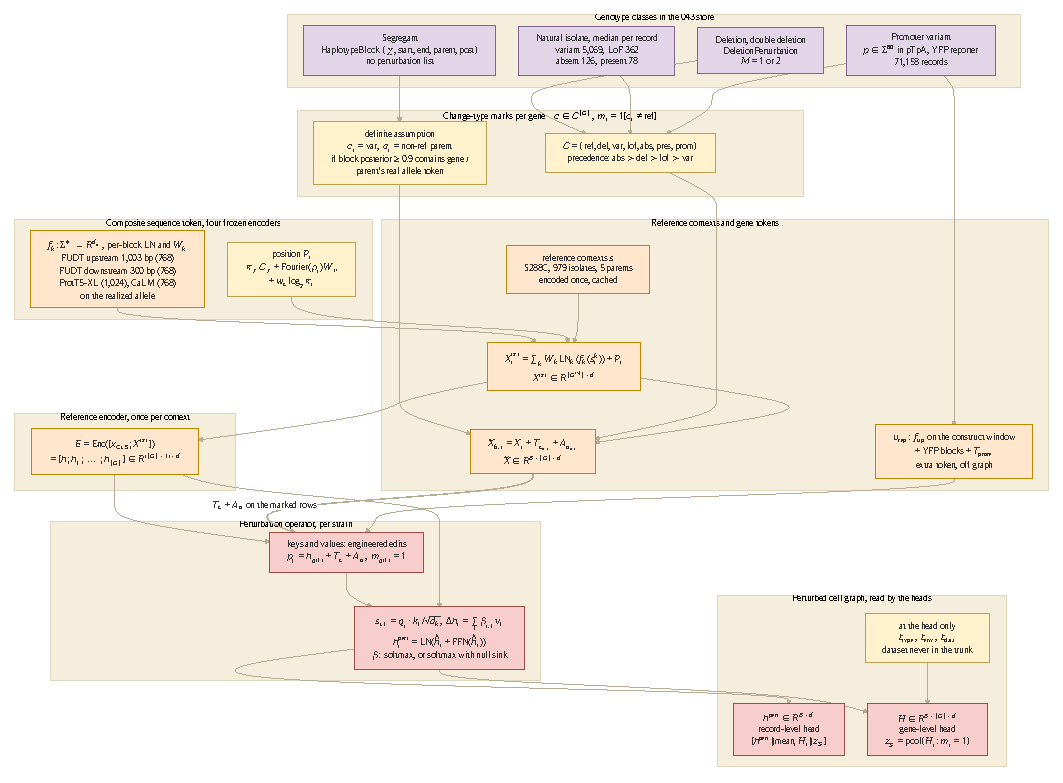
\includegraphics[width=\linewidth,height=0.87\textwidth,keepaspectratio]{figures/mermaid-input-side.pdf}\par\vspace{2pt}
\caption[]{\textbf{Every genotype class reaches the perturbation operator through one
composite sequence token per gene and one encoder pass per reference context.} Top, the
genotype classes and their change-type marks; middle, the four frozen sequence encoders
and the position term, the reference contexts (S288C, each isolate, each non-BY parent)
and their gene tokens, the realized tokens and the reporter token, whose promoter block is
the same FUDT upstream encoder on the construct window; the encoder runs once per context
and is cached; bottom, the operator over the engineered edits and the perturbed states the
heads read, where the type, environment and dataset tokens enter.}
\label{fig:input-side}
\end{figure}
\end{landscape}
%% Generated by notes/assets/publish/scripts/mermaid_pdf.sh from
%% notes/experiments.043-expression-proteome-morphology.mermaid.input-side.md

\subsection{Owner decisions\secstatus{todo}}
\label{sec:input-decisions}

Each item names the recommended option first, then the alternative and the condition under
which it would win. Table~\ref{tab:decisions} carries the same rows with their measured
facts.

\begin{enumerate}
\item \textbf{Base token.} Composite frozen sequence token, Eq.~\ref{eq:input-composite},
with the position term. Alternatives: nucleotide-transformer windows in place of FUDT, for
a host with no FUDT species token (one yeast arm compares the two families now); ESM2 650M
in place of ProtT5 on cost. The identity table is the transductive-ceiling ablation only.
\item \textbf{Absence and deletion.} Two change types; report the cosine of
$T_{\mathrm{del}}$ and $T_{\mathrm{abs}}$ after training.
\item \textbf{Isolates.} Own reference context, operator carries the engineered edits
only (Sec.~\ref{sec:input-isolates}). Alternative: the interim loss-of-function plus
absence mask with allele tokens, if a first run must precede the per-context encoder
(owner question 1).
\item \textbf{Segregant gene membership.} Whole-gene containment, with the parent's actual
allele token on marked genes; all five non-BY parents are collection members.
\item \textbf{Position.} On for every class, Eq.~\ref{eq:input-position}; isolate-own
coordinates deferred to chromosome-scale assemblies.
\item \textbf{Context tokens.} Allele parent on the gene token; environment and ontology
path read by the head (main) or attended after the operator (arm 1); dataset only as the
per-dataset bias at the head, in every arm.
\item \textbf{Normalization at large $M$.} Moot under the main isolate design; softmax;
the sigmoid gate as an arm for the segregant class alone.
\item \textbf{Accessory ORFs and the reporter.} Encode both as extra tokens from the same
encoders; Vaishnav stays in the plan, its linear evaluations run first, and its joint entry
waits on the Addgene 127546 sequence in the constructs tier (owner question 2).
\end{enumerate}

%% notes-tex/multimodal/043-datasets-primer/sections/output-design.tex
%% SOURCE: the numbers are read from notes/experiments.043-expression-proteome-morphology.md
%% (cross_dataset_correlation.py, jobs 5890 and 5892; within_dataset_ceilings.py, jobs 5893,
%% 5895, 5896, 5898; store_census.py), from the 019 campaign write-up on the
%% multimodal-phenotype-retrospective worktree (notes-tex/figure-3-gate/sections/10-data-review.tex
%% and 11-inductive.tex; notes-tex/019-simb-multimodal-expression/sections/2-readouts.tex), from
%% the 035 note (notes/experiments.035-env-chemgen-vanacloig-cgt.md, rounds 9 and 10) and from
%% the Sameith 2015 paper in the mirror (sameithHighresolutionGeneExpression2015/paper.md).
%% The prototype of the heads and the loss is torchcell/models/readout_heads_043.py, tested by
%% tests/torchcell/models/test_readout_heads_043.py; the diagram is
%% notes/experiments.043-expression-proteome-morphology.mermaid.output-side.md.

\section{The output side: readouts, heads, tokens, losses and the evaluation\secstatus{todo}}
\label{sec:output}

What follows is a design for the group to accept, change or reject. The owner's direction
fixes three things: every gene-level readout is trained on; a readout is read off the
perturbed graph, ``from the node itself'' for a gene-level value; and the question to
answer is whether the model improves on held-out Kemmeren single deletions and on the
Sameith double deletions, with Muenzner 2024 as a proteome test and Ohya 2005 CalMorph as a
probe of the learned state and never a training target. Everything else below is a choice
with its facts, Fig.~\ref{fig:output-side} draws the path, and
Sec.~\ref{sec:output-decisions} lists the choices the owner has to make.

%% SOURCE: hand-authored definitions; the numbers in cells cite their section.
\begin{table}[htbp]
\centering
\footnotesize
\caption[]{\textbf{Terms of this section}, alphabetical. Terms of Table~\ref{tab:vocab}
are not repeated.}
\label{tab:output-vocab}
\begin{tabular}{>{\raggedright\arraybackslash}p{30mm}>{\raggedright\arraybackslash}p{140mm}}
\toprule
Term & Meaning \\
\midrule
Additive null & For a double deletion $xy$ and gene $i$, the single-mutant sum
$M_{x,i} + M_{y,i}$, the expected value Sameith 2015 scores its epistasis against
(Sec.~\ref{sec:output-protocol}). It needs no model. \\
Affine, per dataset & A scale $a_k$ and shift $b_k$ applied to a shared head's output for
every record of dataset $k$; $a_k = 1$, $b_k = 0$ at the start. It moves a prediction
between measurement scales and cannot change a correlation. \\
Escape & A run whose training Pearson, in eval mode, passes 0.3. In 019 the genotype-only
morphology runs sat on a plateau at 0.04 to 0.12 that an escape leaves within about 50
epochs (retrospective, \texttt{11-inductive.tex}). \\
Head & The map from a readout site to a predicted value. Joined: one head per readout
type, shared by its datasets. Split: one head per dataset. \\
Perturbed-gene summary $z_S$ & The sum of the perturbed states of the strain's perturbed
genes, $z_S = \sum_{g \in S} H_g$; for a single deletion it is the deleted gene's own
token. The input of the 019 \texttt{M\_zs} readout and of the trigenic-interaction head. \\
Readout site & A tensor of the perturbed graph a head reads: the perturbed CLS $h$, the
summary $z_S$, or the gene states $H$. \\
Readout type & The physical quantity a head predicts: expression log ratio, absolute
expression, expression score, protein abundance, protein turnover, promoter level. \\
Registered window & The epochs over which a run is scored, declared with the epoch budget
before any run of the round is read; 019 used 500 epochs and epochs 400 to 499. \\
Token & A learned vector carried with a record and given to the model: the experiment type
(ontology phenotype class), the dataset, and the environment. \\
\bottomrule
\end{tabular}
\end{table}

%% SOURCE: notes/experiments.043-expression-proteome-morphology.mermaid.output-side.md, rendered by
%% notes/assets/publish/scripts/mermaid_pdf.sh, copied to figures/ by `make diagrams`
\begin{landscape}
\begin{figure}[p]\centering
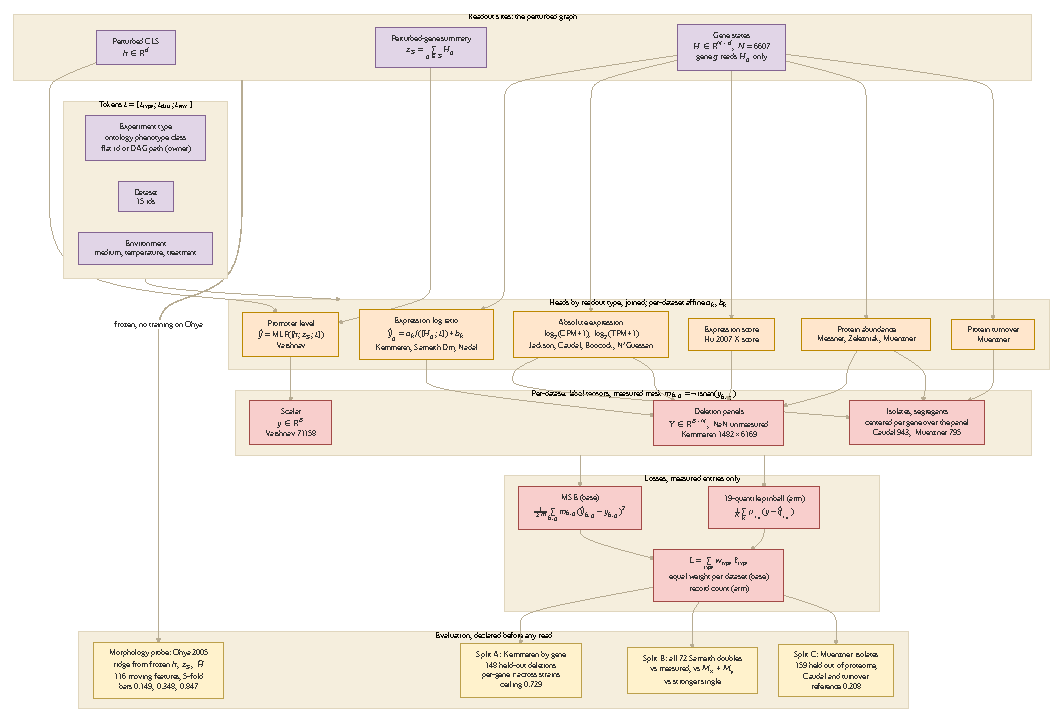
\includegraphics[width=0.92\linewidth]{figures/mermaid-output-side.pdf}\par\vspace{2pt}
\caption[]{\textbf{Gene-level readouts are read from each gene's own perturbed state
through heads joined by readout type, and Ohya is read only from the frozen latent.} Top,
the three readout sites of the perturbed graph; left, the experiment-type, dataset and
environment tokens; middle, the six heads with their per-dataset affines; then the label
tensors with their measured mask and the losses over measured entries; bottom, the
morphology probe and the three held-out splits. Placed on a rotated page at 241 mm,
a scale of 1.14 of the 212 mm rendering.}
\label{fig:output-side}
\end{figure}
\end{landscape}
%% Generated by notes/assets/publish/scripts/mermaid_pdf.sh from
%% notes/experiments.043-expression-proteome-morphology.mermaid.output-side.md

\subsection{Readout sites and the per-gene readout\secstatus{todo}}
\label{sec:output-sites}

The trunk returns three tensors per record after the perturbation operator: the perturbed
class token $h \in \mathbb{R}^d$, the perturbed gene states $H \in \mathbb{R}^{N \times d}$
over the $N = 6{,}607$ gene nodes, and the summary $z_S$. A gene-level value for gene $g$
is read from that gene's own state,
\begin{equation}
\hat y_{g} = a_{k}\, f_\theta\!\big([\,H_g \,;\, t\,]\big) + b_{k},
\qquad t = [\,t_{\mathrm{type}} \,;\, t_{\mathrm{data}} \,;\, t_{\mathrm{env}}\,],
\label{eq:pergene}
\end{equation}
with $f_\theta$ one head shared by every gene and every dataset of the readout type, $t$
the record's tokens (Sec.~\ref{sec:output-tokens}) and $(a_k, b_k)$ the affine of dataset
$k$. The prediction for gene $g$ depends on $H_g$ and on nothing else of $H$; the strain
reaches it through the trunk's attention and the perturbation operator, which is what
``from the node itself'' means in the equation. Four forms of $f_\theta$ are on the table.

\begin{itemize}
\item \textbf{Shared affine.} $f_\theta(x) = w^\top x + c$. The 019 head round measured
the linear per-gene readout within noise of the two-layer one on Kemmeren expression
($+0.002$ over four seeds, \texttt{H\_linear} against \texttt{H\_ref},
\texttt{2-readouts.tex}), so the nonlinearity is not known to carry anything there.
\item \textbf{Shared MLP with per-dataset affine} (Eq.~\ref{eq:pergene}; the prototype
\texttt{PerGeneReadout}). The affine is where the datasets' scales part.
\item \textbf{Shared MLP with the strain vector concatenated.} 019's \texttt{H\_concat}
feeds $[H_g ; c]$ with $c$ the strain context, and was the one arm above the reference in
every seed, $+0.0135$ with a seed sd of $0.0026$ on the difference (\texttt{2-readouts.tex},
Table \texttt{tab:readouts-head}). In Eq.~\ref{eq:pergene} this is $t$ extended by $z_S$.
\item \textbf{Cross-attention head.} One learned query per output feature over every token
(019 \texttt{M\_xattn}). On morphology it escaped under the pinball (4 of 4, $0.121 \pm
0.029$) and not under MSE (1 of 4) (\texttt{11-inductive.tex}). It reads the whole token
set, so it is not a readout from the node itself; it is the alternative if the per-gene
form stalls.
\end{itemize}

A record-level value (Vaishnav 2022, one level per promoter insert) is read from
$[h ; z_S ; t]$ through an MLP, the \texttt{GlobalHead} with \texttt{use\_pert\_summary}
that gave the 019 morphology result (12 of 12 escapes with MSE, $0.149 \pm 0.022$ over the
registered window, \texttt{11-inductive.tex}). The plain CLS escaped 0 of 8 under MSE at
two learning rates, so $h$ alone is not a readout site this design uses for a trained
target; it remains a probe input (Sec.~\ref{sec:output-protocol}).

\subsection{Joined or split heads\secstatus{todo}}
\label{sec:output-heads}

Two facts bound the choice. First, the datasets report different quantities on different
scales (Table~\ref{tab:output-scales}): a two-color $\log_2$ ratio to a wild-type pool, an
error-model X score, a pseudobulk $\log_2$ fold change with sentinels at $\pm 23$ to
$\pm 33$ in 20.2\% of cells (028, \texttt{2-readouts.tex}), UMI counts, TPM, a linear
MaxLFQ abundance, a log SWATH signal, a degradation rate per hour, a sort-seq bin level.
Second, datasets of one quantity agree weakly where they share a genotype
(Table~\ref{tab:cross}): Kemmeren against Hu 0.107, against Jackson 0.043 to 0.076,
against Nadal-Ribelles 0.002 per genotype; Messner against Zelezniak 0.049; Kemmeren mRNA
against Messner protein 0.031. An affine map preserves Pearson, so a per-dataset affine can
reconcile the first fact and cannot reconcile the second: a head shared by two datasets
that agree at 0.002 is asked to emit two unrelated vectors from the same $H_g$, told apart
only by the tokens.

\notesec{Joined by readout type}
Six heads (expression log ratio; absolute expression; expression score; protein abundance;
protein turnover; promoter level), each with one affine per dataset, 15 affines in all. The
datasets that would share a head and the agreement that supports it: Kemmeren and Sameith
Dm (the same arrays and procedures; Sameith's Methods defer to Kemmeren,
Sec.~\ref{sec:between}; the Kemmeren ceiling 0.729 is the only within-type ceiling) and,
under the same head by scale alone, Nadal-Ribelles at 0.002; Jackson, Boocock, N'Guessan
and Caudal under absolute expression (no shared genotype among them; Boocock and N'Guessan
share no segregant, Sec.~\ref{sec:within}); Messner, Zelezniak and Muenzner under protein
abundance (Messner against Zelezniak 0.049; Muenzner shares no genotype with either).
What a joined head buys is the transfer of the readout function across datasets, which is
the premise of the exercise and is unmeasured; what it risks is that a large low-agreement
dataset pulls the shared function away from the one with a ceiling.

\notesec{Split by dataset}
Fifteen heads, no sharing below the trunk. Datasets then meet only in $H$, which is what
every 019 round did with two array datasets (Kemmeren and Sameith) that are the same
arrays. Nothing is known about the trunk's transfer between readout types from this
campaign: proteome from genotype reached $0.085 \pm 0.008$ (v16, 12 runs) and expression
$0.180 \pm 0.006$ (v12, 4 runs) in separate trainings (\texttt{10-data-review.tex}); a joint
training of both was not scored on both.

\notesec{The proposal}
Joined by type with per-dataset affines, under the dataset token, with the two
low-agreement expression datasets (Nadal-Ribelles, Jackson) and Hu switched out as an
arm (Sec.~\ref{sec:output-protocol}). The split design is the control arm of the same
round, not a later step; the paired difference on the Kemmeren held-out score is the
answer. Hypothesis, untested: the affine will absorb the scale and the dataset token will
absorb the dataset's mean profile, leaving the shared head the per-gene response, which is
what transfers.

%% SOURCE: the released-quantity and transform columns are the 043 cross-dataset analysis
%% (notes/experiments.043-expression-proteome-morphology.md, "What each dataset reports");
%% the Nadal sentinel and Vaishnav rows are this section's proposal.
\begin{table}[htbp]
\centering
\scriptsize
\setlength{\tabcolsep}{3pt}
\caption[]{\textbf{Readout type and target transform per dataset.} The transform column is
what the loss sees; ``as released'' means the stored value. The transforms for Jackson,
Caudal, Messner, Zelezniak and Muenzner are the ones the cross-dataset analysis used
(Table~\ref{tab:cross}); the Nadal-Ribelles and Vaishnav rows are proposals.}
\label{tab:output-scales}
\begin{tabular}{>{\raggedright\arraybackslash}p{30mm}>{\raggedright\arraybackslash}p{30mm}>{\raggedright\arraybackslash}p{46mm}>{\raggedright\arraybackslash}p{62mm}}
\toprule
Dataset & Readout type (head) & Released quantity, scale & Target transform \\
\midrule
Kemmeren 2014; Sameith 2015 Dm & expression log ratio & two-color array, $\log_2$ (deletion / WT pool) & as released \\
Nadal-Ribelles 2025 & expression log ratio & pseudobulk $\log_2$ fold change vs WT & as released, with $|{\cdot}| > 20$ set to missing (the zero-mean sentinel; 20.2\% of cells) \\
Hu 2007 & expression score & error-model X score vs BY4741, signed & as released; its own head, since an X score is not a log ratio \\
Jackson 2020 & absolute expression & pseudobulk UMI counts, zeros omitted & $\log_2((\mathrm{CPM}+1)/(\mathrm{CPM}_{\mathrm{HO}}+1))$ against the HO deletion of the same environment, or $\log_2(\mathrm{CPM}+1)$ with the environment token carrying the condition (owner decision) \\
Boocock 2025; N'Guessan 2025 & absolute expression & UMI counts per segregant & $\log_2(\mathrm{CPM}+1)$, centered per gene within the panel \\
Caudal 2024 & absolute expression & RNA-seq TPM, linear & $\log_2(\mathrm{TPM}+1)$, centered per gene over the isolates \\
Messner 2023 & protein abundance & SWATH MaxLFQ, linear & $\log_2$(strain / record reference) \\
Zelezniak 2018 & protein abundance & SWATH log signal (SVA) & strain minus record reference \\
Muenzner 2024 protein & protein abundance & SWATH MaxLFQ precursor quantity, linear & $\log_2$, centered per protein over the isolates \\
Muenzner 2024 turnover & protein turnover & dynamic SILAC degradation rate, per hour & $\log_2$, centered per protein over the isolates \\
Vaishnav 2022 & promoter level & sort-seq expression level, one scalar & standardized over the library \\
\bottomrule
\end{tabular}
\end{table}

\subsection{The experiment-type, dataset and environment tokens\secstatus{todo}}
\label{sec:output-tokens}

Three learned vectors travel with every record. The \textbf{experiment-type token} is the
record's ontology phenotype class: \texttt{Microarray\allowbreak Expression\allowbreak Phenotype} (Kemmeren,
Sameith), \texttt{Microarray\allowbreak Expression\allowbreak Score\allowbreak Phenotype} (Hu),
\texttt{Single\allowbreak Cell\allowbreak Expression\allowbreak Phenotype} (Jackson, Boocock, N'Guessan),
\texttt{Pseudobulk\allowbreak Expression\allowbreak Phenotype} (Nadal-Ribelles), \texttt{RNASeq\allowbreak Expression\allowbreak Phenotype}
(Caudal), \texttt{Protein\allowbreak Abundance\allowbreak Phenotype} (Messner, Zelezniak, Muenzner),
\texttt{Protein\allowbreak Turnover\allowbreak Phenotype} (Muenzner) and \texttt{Pooled\allowbreak Sort\allowbreak Seq\allowbreak Expression\allowbreak Phenotype}
(Vaishnav), the classes of Table~\ref{tab:store}'s rows. The \textbf{dataset token} is the
dataset's id. The \textbf{environment token} is the record's medium, temperature and
environmental perturbation, which separates Jackson's eleven conditions and Nadal-Ribelles'
two.

\notesec{The precedent}
Experiment 035 gave the cell graph transformer a compound token $z_E$ from a fingerprint
MLP and asked whether it predicts Vanacloig 2022 for an unseen compound. Three entry points
were measured on 123 compound-evaluations (\texttt{experiments.035}, rounds 9 and 10): a
bilinear factor at the head ($-0.007$ paired against ridge, 95\% CI $-0.028$ to $+0.015$),
a gate on every gene's state ($-0.025$), and a token the genes attend to for one further
layer ($+0.008$, CI $-0.026$ to $+0.045$; $+0.015$ against the head form, CI through zero).
The ablation was the arm with no compound input (\texttt{cgt\_genes}), whose centered score
is zero by construction. The same three entry points and the same ablation apply here.

\notesec{Where the tokens enter}
(i) At the head only: $t$ concatenated to $H_g$ in Eq.~\ref{eq:pergene} and to $[h ; z_S]$
for the record-level head. Cheapest, and the 035 bilinear form's analog. (ii) On the CLS
row: $t$ added to the class token before the trunk, so every gene can attend to it. (iii)
As a token the genes attend to in one further layer after the perturbation operator, the
035 environment-encoder form, the only one of the three with a positive paired mean
against ridge there. The ablation arm carries no token, and a second ablation carries the
dataset token only, which says whether the experiment type adds anything over the dataset
id (hypothesis, untested: with 15 datasets and 8 classes the two are nearly collinear, and
the type token earns its place only on a dataset unseen in training).

\notesec{Flat id or ontology path}
A flat token is one row per class. A path token sums one row per node of the class's
ontology path, so \texttt{MicroarrayExpressionPhenotype} and
\texttt{RNASeqExpressionPhenotype} share an expression row and differ in their own
(prototype \texttt{ExperimentTypeEmbedding}, \texttt{mode="dag"}). The fact that decides
it: the served graph has no such path. Every phenotype class is a direct child of
\texttt{phenotype} in \texttt{biocypher/config/torchcell\_schema\_config.yaml} (the
\texttt{phenotype member of} edge lists all 34 leaves), and in the pydantic schema only
the two microarray classes share a parent below \texttt{Phenotype}
(\texttt{TwoChannelMicroarrayExpressionPhenotype}). A path token therefore needs a
grouping written on the modeling side (expression, protein, morphology, promoter), or it
waits for the ontology unification to supply one. That is an owner decision
(Sec.~\ref{sec:output-decisions}); the flat token needs nothing new.

\subsection{Losses\secstatus{todo}}
\label{sec:output-losses}

Each readout type has one loss over the measured entries of its records only: a missing
gene is \texttt{NaN} in the target tensor, contributes no value and no gradient, and a type
with nothing measured in a batch returns a connected zero (prototype
\texttt{MaskedTypedLoss}, the convention of \texttt{masked\_mean} in
\texttt{torchcell/losses/distributional.py}). Three choices remain.

\notesec{MSE or pinball}
019 trained expression with the 19-quantile pinball and read the median; on morphology, MSE
on \texttt{M\_zs} escaped 12 of 12 runs by epoch 410 with the smallest spread of any cell,
the pinball on the same readout 8 of 10 and late (epochs 230 to 770), and MSE on the CLS 0
of 8 (\texttt{11-inductive.tex}). The loss and the readout interact, so neither is chosen
for the per-gene heads by that result; the design runs MSE as the default and the pinball
as an arm, both on the per-gene form. The Pearson loss and ListMLE are not arms: five of
six batch-32 Pearson runs collapsed to a constant output and the anchored ListMLE runs sat
on the mean by epoch 250 (\texttt{2-readouts.tex}).

\notesec{Weighting across datasets}
By record the store is 173{,}617 samples, of which Boocock holds 79{,}516 and Vaishnav
71{,}158 (Table~\ref{tab:store}), 87\% of the records in two datasets with no gene-level
deletion genotype; Kemmeren is 1{,}482. A loss averaged over measured entries weights
datasets by records times features, so the deletion panels would be a few percent of the
gradient. Three rules: equal weight per dataset (each dataset's mean loss summed); weight
by the ceiling, so Kemmeren (0.729), Messner (0.696) and Zelezniak (0.916) count more
than Nadal-Ribelles (0.043 against 0.022 across batches) and Jackson (0.129 against
0.095); or by record count. The proposal is equal weight per dataset with the
low-agreement datasets down-weighted by their agreement, and the record-count rule as
the arm that shows what the segregant panels do to the deletion score.

\notesec{Scale}
Every linear quantity is logged before the loss (Table~\ref{tab:output-scales}); every
pair in Table~\ref{tab:cross} was compared log against log, and a correlation does not
depend on the base. Centering per gene over a panel (Caudal, Muenzner, the segregants) is
what the cross-dataset analysis did and is the only way those panels have a zero; it means
their head predicts a deviation from the panel mean, the same object a deletion dataset's
log ratio is.

\subsection{The evaluation protocol\secstatus{todo}}
\label{sec:output-protocol}

Three held-out sets, one probe, four arms and a scoring rule, declared before any run is
read (Table~\ref{tab:output-protocol}).

\notesec{Split A, Kemmeren by gene}
A fraction of Kemmeren's 1{,}482 deletion genotypes, 10\% or 148 genes, is held out by
gene: no record in any deletion dataset whose perturbation set contains a held-out gene is
trained on (Kemmeren, Hu, Jackson, Nadal-Ribelles, Messner, Zelezniak, Ohya), so the gene
is unseen as a perturbation on any readout. A held-out gene still appears in the isolates
and segregants as a sequence variant, an absence or an inherited block; those are not
deletions and are not held out, and an arm without the natural-genome datasets
(below) measures what that leakage, if it is one, is worth. The score is the per-gene
Pearson across the 148 held-out strains for each of the 6{,}169 genes (mean and median
over genes) and the per-strain Pearson across genes (median over strains), both against
the own-culture ceiling 0.729 (test-retest, 114 mutants) and 0.653 (decomposition,
Table~\ref{tab:kemmeren}). The 019 reference on Kemmeren plus Sameith is $0.180 \pm
0.006$ per gene over four runs and 0.233 for one 10{,}000-epoch run
(\texttt{10-data-review.tex}); the 019 split was by strain with the same gene set, so it
is a reference and not a paired bar. The Sameith Sm records are excluded from the store's
training set outright: they are Kemmeren's arrays (82 of 82 identical).

\notesec{Split B, every Sameith double}
All 72 Sameith 2015 double deletions are held out; their constituent singles (82
distinct deletions, the Sameith Sm set) are in training as Kemmeren profiles, so the task
is inference into the combinatorial space from measured singles. Each double is scored against its measured profile (per-strain Pearson
over 6{,}169 genes; per-gene Pearson across the 72 doubles) and paired against two nulls
that need no model: the additive null $M_x + M_y$ from the two Kemmeren singles, which is
the paper's own expected value (``the deviation between the expression change observed in
the double mutant $M_{x\Delta y\Delta i}$ and the expected expression change, given each
single mutant $M_{x\Delta i} + M_{y\Delta i}$'', paper.md line 39), and the stronger
single alone. A third score restricts the genes to those where the double departs from the
additive null by more than the paper's threshold, $|M_{xy,i} - (M_{x,i} + M_{y,i})| >
\log_2 1.5$: on those genes the additive null is wrong by construction and the question is
whether the model is less wrong. Sameith ran ``four times from two independent cultures''
per mutant (paper.md line 33) and released one profile, so no double has a ceiling of its
own; the Kemmeren 0.729 is the bound for the same arrays and procedures.

\notesec{Split C, Muenzner isolates}
A fifth of the 795 Muenzner 2024 proteome isolates, 159, is held out by isolate, and the
same isolates are held out from Caudal 2024 (759 shared) and from the turnover set (55
isolates), so a held-out strain is unseen on every readout. The score is the per-protein
Pearson across the held-out isolates over 1{,}540 proteins and the per-isolate Pearson
across proteins. No Muenzner replicate ceiling is measured (Table~\ref{tab:store}); the
Caudal against Muenzner agreement, 0.208 per isolate and 0.160 per gene
(Table~\ref{tab:cross}), is the reference for what another readout of the same strain
reaches, and the 019 proteome-from-genotype reading on Messner deletions, $0.085 \pm
0.008$, is the reference for the deletion head. Whether an isolate can enter the trunk at
all is the input-side design's question; split C is declared so that the answer has a
test ready.

\notesec{The morphology probe}
Ohya 2005 enters no training. For each of its 4{,}678 genotypes the frozen model produces
$h$, $z_S$ and the mean over genes of $H$; a ridge from each, and from their
concatenation, to the 116 moving CalMorph features is fit 5-fold over genotypes with the
penalty chosen on an inner split, inputs and targets z-scored and clipped at 8, and
scored as the out-of-fold Pearson per feature across held-out genotypes, median over the
116 (the construction of Table~\ref{tab:morph}). The bars, in order: the 019 genotype-only
model read through its own trained head, $0.149 \pm 0.022$; the sequence-embedding ridge
0.08 to 0.14 (\texttt{11-inductive.tex}); the Kemmeren-expression ridge 0.348 on the
1{,}437 shared genotypes and the Messner ridge 0.278 on 4{,}279 (Table~\ref{tab:morph}),
which read the strain's own measurement and are the transductive bars; and the ceiling
0.847 on the 116 features (019) or 0.611 over the 281 (122 wild-type replicates,
Table~\ref{tab:store}). A probe at or above 0.348 from the genotype alone would say the
latent carries what the measured expression carries; one near 0.149 says the probe is the
trained head by another route.

\notesec{Arms}
Four arms in a $2 \times 2$: with and without the natural-genome datasets (Caudal,
Muenzner protein and turnover, Boocock, N'Guessan), with and without Vaishnav; plus the
split-head control and the no-token ablation on the full arm, and the deletion-only
reference (Kemmeren and Messner; Sameith Dm is split B and does not train). Every arm is scored on
splits A, B and the probe; split C exists only in the arms that train isolates. Three
initializations and two split seeds per arm, as 019's v25 (four split seeds, three
initializations) found the escape to be a property of the run and not the split.

\notesec{Window and reads}
The epoch budget and the window are declared with the launch; 019's rule was 500 epochs
read over epochs 400 to 499, declared 2026-10-12, and its 1{,}000-epoch runs scored lower
over 900 to 999 than over 400 to 499 in 7 of 8. A cell is read first by its escape
fraction and second by its window mean; no maximum over epochs is reported. The test
indices of every split are pinned to a file before training and the split-B and split-C
scores are read once, at the end of the round.

%% SOURCE: the n, bar and metric columns cite notes/experiments.043-expression-proteome-morphology.md
%% (store table, cross-dataset and within-dataset sections) and the 019 retrospective.
\begin{table}[htbp]
\centering
\scriptsize
\setlength{\tabcolsep}{3pt}
\caption[]{\textbf{The evaluation protocol.} Every bar is a measured number; a reference is
a number from a different split or model and is marked so.}
\label{tab:output-protocol}
\begin{tabular}{>{\raggedright\arraybackslash}p{18mm}>{\raggedright\arraybackslash}p{44mm}>{\raggedright\arraybackslash}p{22mm}>{\raggedright\arraybackslash}p{44mm}>{\raggedright\arraybackslash}p{42mm}}
\toprule
Split & Held out & n & Metric & Bar \\
\midrule
A, Kemmeren by gene & 10\% of Kemmeren deletion genes; every deletion record naming one, in every deletion dataset & 148 strains, 6{,}169 genes & per-gene Pearson across held-out strains (mean, median over genes); per-strain Pearson across genes (median) & ceiling 0.729 test-retest, 0.653 decomposition; reference 019 by-strain $0.180 \pm 0.006$ \\
B, Sameith doubles & all 72 double deletions; the 82 constituent singles stay in training as Kemmeren records & 72 strains, 6{,}169 genes & per-strain Pearson vs measured; paired difference vs the additive null $M_x + M_y$ and vs the stronger single; the same on genes with $|M_{xy} - (M_x + M_y)| > \log_2 1.5$ & additive null (no model); ceiling 0.729 (same arrays, no double replicate) \\
C, Muenzner isolates & a fifth of the proteome isolates, the same strains out of Caudal and turnover & 159 isolates, 1{,}540 proteins (turnover: those of its 55 among them) & per-protein Pearson across held-out isolates; per-isolate Pearson across proteins & no Muenzner ceiling measured; reference Caudal $\times$ Muenzner 0.208 per isolate, 0.160 per gene; reference 019 Messner $0.085 \pm 0.008$ \\
Morphology probe & Ohya 2005, never trained; 5-fold over genotypes & 4{,}678 genotypes, 116 moving features & ridge from frozen $h$, $z_S$, $\bar H$, their concatenation; out-of-fold Pearson per feature, median over 116 & 019 trained head $0.149 \pm 0.022$; sequence ridge 0.08 to 0.14; Kemmeren ridge 0.348 (1{,}437), Messner 0.278 (4{,}279), transductive; ceiling 0.847 (116) or 0.611 (281) \\
\bottomrule
\end{tabular}
\end{table}

\subsection{Owner decisions\secstatus{todo}}
\label{sec:output-decisions}

\begin{enumerate}
\item \textbf{Joined or split heads.} Joined by readout type with per-dataset affines (six
heads, 15 affines), or one head per dataset (15 heads). Facts: same-type agreement is
0.002 to 0.107 for expression and 0.049 for protein (Table~\ref{tab:cross}); an affine
cannot raise a correlation; no joint training across types has been scored. Proposal:
joined, with split as the control arm.
\item \textbf{Flat or path token for the experiment type.} The served ontology is flat
(34 leaves under \texttt{phenotype}); a path needs a modeling-side grouping or the
unification. Proposal: flat now, path when the ontology carries one.
\item \textbf{Where the tokens enter.} Head only, CLS row, or attended token (035's three
forms; $-0.007$, $-0.025$, $+0.008$ against ridge, all CIs through zero). Proposal: head
only as the base, attended token as the arm.
\item \textbf{Loss.} MSE or the 19-quantile pinball on the per-gene heads (019: MSE on
$z_S$ 12 of 12 escapes, pinball 8 of 10, on morphology only). Proposal: MSE base, pinball
arm.
\item \textbf{Dataset weighting.} Equal per dataset, by ceiling, or by record count (two
datasets hold 87\% of the records). Proposal: equal per dataset, agreement-weighted for
the low-agreement sets, record count as an arm.
\item \textbf{Nadal-Ribelles sentinels.} Treat $|\log_2 \mathrm{FC}| > 20$ as missing
(20.2\% of cells), or keep the stored value. Proposal: missing.
\item \textbf{Jackson target.} Deletion effect against the HO control of the same
environment, or the absolute $\log_2(\mathrm{CPM}+1)$ with the environment token carrying
the condition. Facts: construction pairs agree at 0.129 against 0.095 on the effect, and
one genotype across environments at 0.010. Proposal: the effect.
\item \textbf{Split A leakage rule.} Hold the gene out of every deletion dataset (proposed)
or out of the expression datasets only; the natural-genome arm measures the isolate and
segregant side either way.
\item \textbf{Split C size and existence.} A fifth of the isolates held out, contingent on
the input-side design admitting isolates at all.
\item \textbf{Budget and window.} Epochs and window to declare with the launch; 019's 500
and 400 to 499 are the precedent.
\end{enumerate}


\end{document}
